\documentclass[a4paper]{report}

\usepackage{times}
\usepackage{graphicx}
\usepackage{amsmath,amssymb}

% Any macro definitions you would like to include
% These are not defined in the style file, because they don't begin
% with \bmva, so they might conflict with the user's own macros.
% The \bmvaOneDot macro adds a full stop unless there is one in the
% text already.
\def\eg{\emph{e.g.,}}
\def\ie{\emph{i.e.,}}
\def\etal{\emph{et al.}}
\def\vs{\emph{vs.}}

% macros for referencing figures, tables, equations and sections
\newcommand{\fref}[1]{Figure~\ref{#1}}
\newcommand{\eref}[1]{(\ref{#1})}
\newcommand{\tref}[1]{Table~\ref{#1}}
\newcommand{\sref}[1]{Section~\ref{#1}}
\newcommand{\aref}[1]{Algorithm~\ref{#1}}
\newcommand{\emptybox}[2]{\framebox[#1][l]{\rule[#2]{0pt}{0pt}}}

% maths macros
\def\G{G}
\def\Gx{G_x}
\def\Gy{G_y}
\def\Gxx{G_{xx}}
\def\Gxy{G_{xy}} \def\Gyx{G_{yx}}
\def\Gyy{G_{yy}}
\def\Ix{I_x}
\def\Iy{I_y}
\def\Ixsqr{I_{x^2}}
\def\Iysqr{I_{y^2}}
\def\Ixx{I_{xx}}
\def\Ixy{I_{xy}}
\def\Iyy{I_{yy}}
\def\dtcwt{DT-$\mathbb{C}$WT}

\def\deg{$^\circ$}
\def\by{{\times}}

% lengths for image sizes
\newlength{\qtrcol}
\setlength{\qtrcol}{0.21\columnwidth}

% command for adding inline comment to text
\newcommand{\comment}[1]{}

% define title here so headers are updated, too
\def\ttl{Estimating Orientation of Curvilinear Structure}
\title{\ttl}
\author{Authors}

% define path to figures
\def\figroot{./figs}
\def\figpath{\figroot}


%-------------------------------------------------------------------------
% Document starts here
\begin{document}

\maketitle

\begin{abstract}
Estimating orientation of image structure underpins applications including digital mammography, retinography and fingerprint analysis. We consider different choices of filter bank including those based on first and second derivatives, efficient Haar-like features and the Dual Tree Complex Wavelet Transform. We then investigate how standard regressors (linear regression, Boosting and Random Forests) may be adapted to use the responses to these filter banks in order to predict orientation of image structure. For a quantitative evaluation, we use synthetic images based on mammograms and the publicly available DRIVE database of retinal images, and show that Random Forests and the wavelet transform offer superior accuracy though at a cost in efficiency. Qualitative results are also presented for real mammograms and fingerprint images.
\end{abstract}

\section{Introduction}
\begin{itemize}
\item We begin by discussing the two techniques most important to this study: the Dual Tree Complex Wavelet Transform; and Random Forests.

\item We then show that these can be used to detect curvilinear structure in images

\item We then show that they can be used to distinguish between different types of curvilinear structure (via a classifier)

\item We also show that similar techniques can be used to estimate orientation, which is useful in a number of applications.
\end{itemize}

% General purpose image processors such as Gaussian 2nd derivatives work pretty well and can be applied to any image
% Since we know that we are using a particular type of image, however, we expect that methods tailored to our specific application will work better. We therefore investigate Machine Learning methods based on labelled training data, that can capture specific properties (e.g. noise characteristics) of our problem domain.

%Breast screening programmes using x-ray mammography have been deployed widely to detect early signs of cancer. The use of computer-aided detection systems to support breast radiology experts is also widespread. In mammograms, the projection of a complex network of vessels, ducts and connective tissue in the breast results in images that are rich in linear structures at a variety of scales and orientations. Mammographic signs of cancer include: the presence of a radio-opaque mass, often with associated radiating curvilinear structures (spicules); the presence of microcalcifications (clusters of highly radio-opaque 'dots'); and the presence of abnormal or abnormally organised curvilinear structures (architectural distortion - AD). Fig 3(a) shows an approximately 4 x 4 cm region extracted from a mammogram, centred on a malignant tumour, and demonstrates a central mass and radiating spicules, along with normal curvilinear structures (vessels, ducts, glandular tissue etc). The signs of abnormality often appear in conjunction, but when only AD is present, detection of the abnormality is extremely difficult. It has been estimated that approximately a third of all cancers missed during mammographic screening present as AD [3], and it has been reported that computer-aided detection systems do not yet detect AD with adequate sensitivity or specificity [4].
%
%Previous attempts at detecting both patterns of spicules associated with malignant masses and more general distortions in which no focal mass is visible have employed a two stage approach comprising i) the detection of all curvilinear structures in a specified region, ii) an analysis of the orientation pattern of the detected structures to determine whether abnormal patterns are present [5-7]. The work we report here seeks to provide a firmer foundation for this approach by improving the detection of curvilinear structures and identifying those structures likely to be (abnormal) spicules.


\section{Background}
We conduct experiments in three domains: line detection, line classification, and orientation estimation.

Detecting curvilinear structure in an image (\eg~roads and rivers in aerial images, cracks in manufactured components, blood vessels and ducts in medical images) is difficult because these structures often appear at relatively low contrast against a cluttered background. To separate the meaningful structure from the background clutter, we adopt a discriminative learning approach based on the \dtcwt~\cite{Kingsbury_ACHA01} for local image representation and Random Forests~\cite{Breiman_ML01} for classification. This approach achieves high detection accuracy by taking account of the domain-specific characteristics of both the structures of interest and the background clutter.


\section{Conclusions}
From these experiments, we can make several conclusions. First, we see that filters based on first derivatives do indeed perform poorly near the centre of a ridge feature (\fref{f:fingerprints}b); second derivatives are much better, though they result in artefacts at the edges (where we are less concerned). Second, there is potential to approximate the second derivative filter responses with Haar-like features if efficiency is a key concern, though it is less clear how to combine these responses to give a unique solution. Of the filters we tested, we found that the \dtcwt~gave the best results regardless of the regressor used, though was significantly more computationally expensive. Of the regressors we tested, Random Forests performed best and we have provided some insight as to why alternatives (\eg~linear regression) perform less well. We must, however, take care when building regressors for orientation prediction in order to ensure that angles wrap around the circle correctly.


\section{Output definition}
[Describe here how the outputs of the regression are defined \ie~double-angled complex vector form. We'll need this early on so that the reader knows by the time we talk about the Random Forest regression. It could alternatively come between the image representation (inputs) and RF regression.]

\chapter{Techniques}

\section{Image Representation}
\label{s:filtering}
To predict some quantity (\eg~line probability, line orientation) from an image sample, it is useful to reduce the high-dimensional image data to a more compact feature vector that captures the most important properties of the image and discards redundant information. This reduces the effects of the `curse of dimensionality'~\cite{Bellman} whereby the number of training examples required for a given sampling density increases exponentially with input dimensionality, and improves the performance of statistical pattern recognition algorithms. This section gives an overview of some of the available options.

\subsection{Template Matching}
Early attempts at detecting linear structure in an image used modifications of template matching (such as the Line Operator, or `LinOp'~\cite{Dixon_Taylor_IPC79}), applying a template at multiple scales and used the orientation and scale (and possibly response) as the features used to describe an image patch. 

% Mammography examples
Though originally applied to detecting asbestos fibres, it was later shown that LinOp could be na\"ively applied to mammograms~\cite{Parr_etal_SPIE97}. Other approaches to detecting linear structure in mammograms include using second derivatives of the mammographic image surface~\cite{Cerneaz_Brady_CVVRRM95} or second derivatives of the 2D Gaussian~\cite{Karssemeijer_teBrake_TMI96}. In a comparison of these methods that used simulated mammograms~\cite{Zwiggelaar_etal_TMI04}, LinOp achieved the best results in terms of maximizing the area under the receiver operating characteristic (ROC) curve.


\subsection{First derivatives}
A simple but na\"ive filtering approach uses smoothed derivatives, $\Gx$ and $\Gy$ (\fref{f:filters}a-b), and their corresponding responses, $\Ix$ and $\Iy$, to compute the direction in which gradient is strongest; the perpendicular to this gradient defines the line orientation.

Defining $\G_{(1)}(\theta)$ as the first derivative filter at angle $\theta$,
%
\begin{align}
G_{(1)}(\theta)
	&= 	\frac{\partial G}{\partial r} \\
	&= 	\frac{\partial G}{\partial x}\frac{\partial x}{\partial r} +
			\frac{\partial G}{\partial y}\frac{\partial y}{\partial r} \\
	&= 	\Gx \cos(\theta) + \Gy \sin(\theta)
\label{e:dG}
\end{align}

\noindent where $\Gx = G_{(1)}(0^\circ)$ and $\Gy = G_{(1)}(90^\circ)$. The response to this filter is
%
\begin{align}
R_{(1)}(\theta)
	&= 	\G_{(1)}(\theta) \ast I \\
	&=	(\Gx \cos(\theta) + \Gy \sin(\theta)) \ast I \\
	&=	(\Gx \ast I) \cos(\theta) + (\Gy \ast I) \sin(\theta) \\
	&=	\Ix \cos(\theta) + \Iy \sin(\theta)
\label{e:R1}
\end{align}

\noindent where $\Ix$ and $\Iy$ are the responses to $\Gx$ and $\Gy$, respectively. That the response at any $\theta$ is a linear sum of the response at two orientations is the property of \emph{steerability} that makes computing the response at any angle efficient. Differentiating and equating to zero gives
%
\begin{align}
\frac{d}{d\theta}R_{(1)}
	&= -\Ix \sin(\theta) + \Iy \cos(\theta) = 0 \\
\Rightarrow \tan(\theta)
	&= \frac{\Iy}{\Ix}.
\label{e:t1}
\end{align}

One problem with this approach is that although the gradient has a clear direction (\eg~dark to light) its perpendicular does not: there are two opposite directions, both with zero gradient, and the estimated orientation is arbitrary up to a rotation of $180^\circ$. Though technically we do not distinguish between opposite orientations, opposites cancel when computing statistics (\eg~the mean orientation over a local patch). 


\subsection{Squared responses}
This problem can be avoided by considering the squared response to $G_{(1)}(\theta)$:

\begin{align}
R_{(1)}^2(\theta)
	&=	(\Ix \cos(\theta) + \Iy \sin(\theta))^2 \\
	&= 	\Ix^2 \cos^2(\theta)+\Iy^2 \sin^2(\theta)+2\Ix\Iy\sin(\theta)\cos(\theta) \\
	&= 	\Ix^2 \cos^2(\theta)+\Iy^2 \sin^2(\theta)+\Ix\Iy\sin(2\theta)
\label{e:R1sqr}
\end{align}

\noindent such that differentiating and equating to zero gives
%
\begin{align}
\frac{d}{d\theta}R_{(1)}^2
	&= 	-2\Ix^2 \cos(\theta)\sin(\theta) + 2\Iy^2 \sin(\theta)\cos(\theta) + 2\Ix\Iy\cos(2\theta) \\
	&= 	(\Iy^2-\Ix^2) \sin(2\theta) + 2\Ix\Iy\cos(2\theta) = 0 \\
\Rightarrow \tan(2\theta)
	&= 	\frac{2\Ix\Iy}{\Ix^2-\Iy^2}.
\label{e:t1sqr}
\end{align}

\noindent where, by doubling the angle, opposite orientations reinforce each other rather than cancel out~\cite{Mardia_Jupp_00}. 


%\subsection{Squared filters}
%\begin{align}
%\tan(2\theta)
%	&= 	\frac{2(\Gx\Gy \ast I)}{(\Gx^2 \ast I)-(\Gy^2 \ast I)}.
%\label{e:t1fsqr}
%\end{align}
%
%\noindent with `cloverleaf' type filters.


\subsection{Second derivatives}
A further criticism of the first derivative approach is that $\Gx$ and $\Gy$ respond most strongly at the edges (rather than the centre) of a bar. In fact, any approach based on odd image filters (including the monogenic signal~\cite{Felsberg_Sommer_TSP01}) fails at the centre of symmetric bar features where both $\Ix$ and $\Iy$ are close to zero such that line orientation is poorly defined. Taking products of the responses does not help in this respect -- the products are also close to zero -- but filters based on second derivatives (and that are therefore even) can provide a more stable solution.

We define $\G_{(2)}(\theta)$ as the second derivative filter at angle $\theta$ such that

\begin{align}
\G_{(2)}(\theta)
	&= 	\frac{\partial}{\partial x}(\Gx \cos(\theta) + \Gy \sin(\theta))\frac{\partial x}{\partial r} \notag\\
		&\qquad + \frac{\partial}{\partial y}(\Gx \cos(\theta) + \Gy \sin(\theta))\frac{\partial y}{\partial r} \\
%
	&= 	(\Gxx \cos(\theta) + \Gyx \sin(\theta))\cos(\theta) \notag\\
		&\qquad + (\Gxy \cos(\theta) + \Gyy \sin(\theta))\sin(\theta) \\
%
	&= 	\Gxx\cos^2(\theta) + \Gyy\sin^2(\theta) + 2\Gxy\sin(\theta)\cos(\theta) \\
%
	&=	\Gxx\cos^2(\theta) + \Gyy\sin^2(\theta) + \Gxy\sin(2\theta)
\label{e:ddG}
\end{align}

As noted some years ago (and exploited in mammography applications~\cite{Karssemeijer_teBrake_TMI96}), second derivatives are also steerable and are therefore highly efficient~\cite{Freeman_Adelson_TPAMI91,Koenderink_vanDoorn_TPAMI92}. For further efficiency, we differentiating $\Gx$ and $\Gy$ to get the equivalent \emph{separable} filters $\Gxx$, $\Gyy$ and $\Gxy$ (\fref{f:filters}c-e), and use these to compute the response to $G_{(2)}(\theta)$,

\begin{align}
R_{(2)}(\theta)
	&= 	\G_{(2)}(\theta) \ast I \\
	&=	\Ixx\cos^2(\theta) + \Iyy\sin^2(\theta) + \Ixy\sin(2\theta).
\label{e:R2}
\end{align}

\noindent where $\Ixx$, $\Iyy$ and $\Ixy$ are the responses to $\Gxx$, $\Gyy$ and $\Gxy$, respectively. If we differentiate with respect to $\theta$, we find a stationary point at

\begin{align}
\frac{d}{d\theta}R_{(2)}
	&= 	-2\Ixx\cos(\theta)\sin(\theta) + 2\Iyy\sin(\theta)\cos(\theta) + 2\Ixy\cos(2\theta) \\
	&= 	(\Iyy-\Ixx)\sin(2\theta) + 2\Ixy\cos(2\theta) = 0 \\
\Rightarrow \tan(2\theta)
	&= 	\frac{2\Ixy}{\Ixx-\Iyy}.
\label{e:t2}
\end{align}

Since \eref{e:t1sqr} and \eref{e:t2} actually give values of $2\theta \pm k\pi$, solving for $\theta$ gives two orientations (one minimum and one maximum) that are $90^\circ$ apart. An analytic solution then requires us to compute the actual response at the two solutions in order to estimate line orientation. 


\subsection{Haar-like Approximations}
At this point it is helpful to examine the equivalent filters involved: $\Ixy$ and $\Ixx-\Iyy$ (\fref{f:filters}e,f). In particular, we note that their distinctive `cloverleaf' appearance is well approximated by highly efficient Haar-like features (\fref{f:filters}g,h) that have demonstrated success since their introduction for face detection~\cite{Viola_Jones_IJCV04}. To approximate $\Gxx-\Gyy$, we used a modification of the summed area table to compute features at $45^\circ$~\cite{Lienhart_Maydt_ICIP02}.

\begin{figure}[t]
\centering
\begin{tabular}{c c c c}
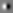
\includegraphics[width=0.15\columnwidth]{\figpath/Gx} &
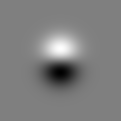
\includegraphics[width=0.15\columnwidth]{\figpath/Gy} &

\includegraphics[width=0.15\columnwidth]{\figpath/Gxx} &
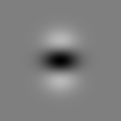
\includegraphics[width=0.15\columnwidth]{\figpath/Gyy} \\
(a) & (b) & (c) & (d) \\
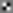
\includegraphics[width=0.15\columnwidth]{\figpath/Gxy} &

\includegraphics[width=0.15\columnwidth]{\figpath/Gxx-Gyy} &

\includegraphics[width=0.15\columnwidth]{\figpath/haar_sin} &

\includegraphics[width=0.15\columnwidth]{\figpath/haar_cos} \\
(e) & (f) & (g) & (h) \\
\end{tabular}
%
\caption{(a,b)~First derivatives, $\Gx$ and $\Gy$; (c-e)~Second derivatives, $\Gxx$, $\Gyy$ and $\Gxy$; (f)~$\Gxx-\Gyy$; (g,h)~Haar-like approximations to $\Gxy$ and $\Gxx-\Gyy$.}
\label{f:filters}
\end{figure}


\subsection{The Dual Tree Complex Wavelet Transform (\dtcwt{})}
Although filters based on second derivatives can give accurate output when positioned at the centre of a line feature, accuracy when away from the centre of the line cannot be assured. It has been noted, therefore, that accommodating variation in \emph{phase} of the filter can offer benefits in this regard. 

In particular, researchers have recognised the importance of using local phase information to distinguish between strong edges and genuine curvilinear structure. In mammography, examples include using Gabor filters~\cite{Rangayyan_Ayres_MBEC06}, while other studies used sets of complex filters~\cite{Schenk_Brady_IWDM02,McLoughlin_etal_SPIE02} that were also steerable~\cite{Freeman_Adelson_TPAMI91}, at multiple scales to compute local energy, orientation and phase at each pixel. One further study used the `monogenic' signal~\cite{Wai_etal_MICCAI04} as a more efficient way of calculating local phase and orientation at multiple scales, detecting curvilinear structure using amplitude-weighted local phase congruency. Overall, the conclusion that can be drawn from the literature is that the detection of curvilinear structure benefits from access to local phase and magnitude information at multiple scales.

An alternative to these methods is to use wavelets to describe the underlying image information. Wavelet transforms have been used extensively in image processing and analysis to provide a rich description of local structure. In particular, the Dual-Tree Complex Wavelet Transform (\dtcwt{}) gives a directionally selective representation that combines the computational efficiency of decimation (\ie~multiresolution filtering is achieved by successively down-sampling the image than by increasing filter size) with approximately shift-invariant coefficient magnitudes and local phase information~\cite{Kingsbury_ACHA01}. The \dtcwt{} combines the outputs of two discrete transforms, using real wavelets differing in phase by 90\deg, to form the real and imaginary parts of complex coefficients. For 2-D images, it produces six directional sub-bands, oriented at $\pm$15\deg, $\pm$45\deg and $\pm$75\deg, at each of a series of scales separated by factors of two. The DT-CWT is less expensive to compute and provides a richer description (magnitude and phase at six orientations rather than one) than the monogenic signal~\cite{Wai_etal_MICCAI04}.

Though it is easy to argue for the rich description of local structure provided by the \dtcwt{}, we must decide how to use this information to compute a single measure of curvilinear structure probability. One solution would be to select the maximum of the six oriented sub-band coefficients at each scale, and combine them across scale in a measure of phase congruency, as in the monogenic signal based method~\cite{Wai_etal_MICCAI04}, but this would discard potentially useful information. Instead, we pose the problem as a classification task in which we attempt to learn the patterns of DT-CWT coefficients associated with pixels belonging to either linear structures or background. 

We construct a feature vector characterising each pixel by sampling \dtcwt{} coefficients (in phase/magnitude form) from the six oriented sub-bands in each of the $s$ finest decomposition scales from a neighbourhood centred on the pixel. This involves interpolating the coefficients obtained at coarse scales to provide a response at every pixel using a band-pass interpolation method~\cite{Anderson_etal_ICIP05}. 

To improve further the rotational symmetry of the coefficients, we also apply an additional set of filters to reduce the wave frequencies of the 45\deg and 135\deg sub-bands so that they lie closer to the 15\deg, 75\deg, 105\deg and 165\deg bands~\cite{Kingsbury_ECSP06,Berks_etal_IPMI11}. The six sub-bands are then multiplied by \{$i$, -$i$, $i$, -1, 1, -1\} respectively, so that the phase at the centre of the impulse response of each wavelet is zero. Finally, to achieve 180\deg rotational symmetry, we replace any coefficient with negative imaginary part with its complex conjugate (equivalent to taking the absolute value of the local phase).

When dealing with a complex response, $c$, we separate its magnitude, $|c|$, from its phase, $\angle c$. Since orientation is only defined up to a rotation of $180^\circ$, however, a point with phase $\phi$ displaced by $d$ from the centre of a line is indistinguishable from a point with phase $-\phi$ displaced by $-d$ from the same line when looking in the opposite direction; we therefore take the absolute value of phase, $|\angle c|$, at each pixel.


\subsection{Multiresolution Filtering}
Since curvilinear structure appears at a number of scales in the image (\eg~from fine spicules to thick ducts in mammograms), it is also important to filter the image at several scales to capture all structure~\cite{Lindeberg_IJCV98b}. Having applied our filter bank at a number of scales, an important question is how to interpret the responses at each scale. One option is to discard all scales but that with the strongest overall response~\cite{Karssemeijer_teBrake_TMI96} and use the responses from the discrete orientations at the selected scale to determine orientation analytically. In this work, however, we investigate the alternative approach whereby we use the responses at all scales as input to a regressor that predicts the orientation directly. This general purpose approach has the added advantage that it can be applied for filter banks where an analytic solution is not obvious (such as the \dtcwt{}).
\section{Classification}
Whichever representation we choose, we end up with a vector of features from which we want to predict either a classification label (e.g. vessel vs. non-vessel, spicule vs. non-spicule) or a real number (e.g. line orientation).


If we have examples of labelled image data for which we wish to estimate orientation, a sensible approach is to compute filter responses (\ie~that form a feature vector) at sampled points in these images and train a regressor to predict the corresponding orientation. We can then apply the trained regressor to a previously unseen image in order to estimate orientation in new cases. Not only is this approach beneficial where an analytic solution is not obvious (as in the \dtcwt{}) but can also account for factors such as the expected distribution of line widths in a typical image and non-Gaussian noise in medical imaging applications. For the three regressors we use, the targets that we predict are a unit vector in the complex plane where the angle has been doubled (\ie~$t_k = \cos 2\theta_k + i\sin 2\theta_k$) to avoid ambiguity over direction~\cite{Mardia_Jupp_00}. Furthermore, for each pixel we define the feature vector as the responses to all filters pooled over the surrounding $3{\times}3$ pixel region.


\subsection{Linear Regression}
\label{s:learning_linear}
The simplest approach uses a linear regressor such that the predicted output is a weighed sum of the filter responses. Because the outputs are complex the regression coefficients are complex also, though this problem is equivalent to regressing over $\cos 2\theta$ and $\sin 2\theta$ independently.
%Under ideal conditions, applying this method to the real filters (\eg~first and second derivatives) should produce regression coefficients identical to those computed analytically.\comment{Not sure if that is entirely relevant}

%Since the linear regressor minimizes the mean squared error (in $\cos 2\theta$ and $\sin 2\theta$), the uncertainty in the prediction can be represented as an axis aligned Gaussian distribution in the complex plane. If the errors are equally distributed for both $\cos 2\theta$ and $\sin 2\theta$ -- and our experience suggests that they are typically close -- then the angular error (\ie~the angle subtended by isocontours of the Gaussian) is constant for an input of given magnitude; uncertainty is proportionally lower for inputs with larger magnitude, and vice versa. Since phase is limited to the range $[-\pi,\pi)$, however, the magnitude of the feature vector is strongly correlated with the magnitude (rather than phase) of the response to the \dtcwt{}. As a result, image features with high contrast that respond strongly to the \dtcwt{} have lower relative uncertainty (an intuitive result).\comment{This could be considered as 'discussion' and may not be relevant right here}


%\subsection{Logistic Regression}
%\label{s:learning_logistic}
%Since we are predicting sin2T and cos2T, it makes sense to apply some limits to the values these can take. One possibility is to us logistic regression (usually used for classification) which can model a linear region for appropriately scaled targets or a sigmoidal output if necessary. We scale sin and cos to the range [0,1] to learn the regressor and apply the reverse transform on the predictions. This does not restrict outputs to be on (or within) the unit circle but within the unit square.
%
%This is slower to train since it requires iteratively reweighted least squares to minimize the objective function though adds little to testing times.
%Uncertainty will be tricky here


\subsection{Boosted Regression}
\label{s:learning_boosted}
Though straightforward, linear regression breaks down if the relationship between inputs and outputs is in fact nonlinear. Furthermore, the output of a linear regressor is unbounded even though in reality $-1 \leq \sin\theta,\cos\theta \leq 1$. We therefore investigate additive (or \emph{boosted}) regression models that can not only limit output but also capture any nonlinearities in the relationship between feature vector and orientation.

In this work we use an additive model composed of $N=100$ piecewise constant functions. To train the model, we start with a zero residual and iterate the following steps $N$ times: fit a weak predictor to each dimension of the training data in turn; select the dimension and corresponding predictor that minimize the residual error; add a fraction (we use $0.05$) of the prediction to the estimated outputs -- a process known as \emph{shrinkage}~\cite{Friedman_AoS01}; and recompute the residual error. This boosting process is thought to be more insensitive to overtraining than most Machine Learning methods.


\subsection{Random Forest Regression}
\label{s:learning_forest}
Random forests have been shown to be capable of learning complex nonlinear relationships over large numbers of variables (with absolute scales that are incommensurate) at a reasonable computational cost~\cite{Breiman_ML01}. Furthermore, they require little or no tuning and are often resistant to overtraining, making them ideally suited to our regression task. We must be cautious, however, when using trees to predict orientation where vectors close to each other in the complex plane (\eg~$-1+\epsilon i$ and $-1-\epsilon i$) may be confused as being far apart based on their angle alone.

Moreover, splitting dimensions and thresholds are usually chosen based on the variance of the sample either side of the threshold under the assumption of a input Euclidean space. As this assumption does not apply to orientation vectors, we instead use the angular dispersion~\cite{Mardia_Jupp_00}: for a sample of $N$ orientations $\{\theta_k\}$, represented in angle-doubled vector form as $t_k = \cos 2\theta_k + i\sin 2\theta_k$, the angular dispersion, $D$, of the sample can be defined as the magnitude of the mean vector over the sample,
%
\begin{equation}
D = |\frac{\sum{t_k}}{N}|.
\label{e:2d}
\end{equation}

By definition, $D$ reaches its maximum of 1 when all $t_k$ are equal, and its minimum of 0 when orientations are distributed uniformly about the circle or when the sample consists of pairs exactly $180^\circ$ apart. The aim of each regression tree is to find parts of the input feature space that are associated with pure samples of orientation. Thus we implement our splitting criteria such that the sum of the angular dispersions of the two samples produced by the split is maximised.

We have found, however, that rather than constructing trees until completely pure leaves are found (\ie~nodes with $D$ arbitrarily close to 1), it is both computationally more efficient and more robust to stop when some minimum leaf size is reached (typically 0.05\% of the total input samples). We then store the mean sample vector of orientations at each leaf, in effect encoding a summary description of the sample of orientations at that point in feature space. The magnitude of these vectors can be viewed as the confidence in a leaf's ability to predict orientation. 

When we come apply the regression forest to predict orientations, we take the mean of the predictions from the individual trees. As a result, trees which described the input feature poorly (and thus return a leaf orientation vector with small magnitude) contribute little to the overall orientation prediction, relative to trees that were able to match the input feature to a pure sample of orientations. Implementing forests in this way produces orientation predictions that are both more accurate and more robust (\ie~resistant to overtraining) than those from unpruned trees with uniform weighting. 

Finally, the magnitude of the prediction gives a measure of the forest's confidence in the prediction. Not only could this serve as a substitute for curvilinear structure detection, but is also useful for weighting predictions in visualization (see \fref{f:real_mammography}). 
%Previous work has looked at detecting structure by applying random forest classifiers to \dtcwt{} based feature vectors and we are currently exploring the link between two. \comment{ possibly cite our earlier work or reyhaneh's stuff - I promise I'm not doing this just self cite, it seems genuinely relevant!}


\comment{
\item When estimating orientation with a tree (or forest of trees), there is a particular problem when the output is limited to a specific range e.g. (0,2pi]. At the two extremes of the range, samples in the bins near the end are biased toward the centre of the range such that, in our case, it is very unlikely that a 0 or 2pi will be output by the forest.
Random Forests (or trees for that matter) have the option of giving us a multimodal distribution over orientation which will be useful at points where lines cross.
One advantage of the (pruned) tree approach is that each bin contains a number of training samples such that we can estimate a mean value and an uncertainty (variance) for every leaf. In other words, the variance is very much data dependent.
This then propagates in the case of a Random Forest since the individual tree outputs can be combined with their respective variance accounted for correctly.
The output from the Random Forest is always between 0 and 1 in magnitude. Question: should we be taking the square root of the complex vector to halve the angle (and therefore sqrt the magnitude also)? At the moment, vectors are weighed by their unsquared magnitude.
}

\section{Random Forests}
Random forest classifiers have become popular because of their ease of use (rapid training, no critical parameters to select), resistance to overtraining, and near state-of-the-art performance. Given a set of training data consisting of N samples, each of which is a $D$-dimensional feature vector labelled as belonging to one of $C$ classes, a random forest comprises a set of tree predictors constructed from the training data~\cite{Breiman_ML01}. Each tree in the forest is built from a bootstrap sample of the training data (that is, a set of $N$ samples chosen randomly, with replacement, from the original data). The trees are built using a standard classification and regression tree (CART) algorithm; however, rather than assessing all D dimensions for the optimal split at each tree node, only a random subset of $d < D$ dimensions are considered. The trees are built to full size (\ie until a leaf is reached containing samples from only one class) and do not need to be pruned (although they can be for the sake of efficiency).

During classification, an unseen feature vector is classified independently by each tree in the forest; each tree casts a unit class vote, and the most popular class can be assigned to the input vector. Alternatively, the proportion of votes assigned to each class can be used to provide a probabilistic labelling of the input vector. Random forests are particularly suited to learning non-linear relationships in high-dimensional multi-class training data, and have been shown to perform as well as classifiers such as Adaboost or support vector machines, whilst being more efficient to compute~\cite{Breiman_ML01}.

Similarly, by building regression rather than classification trees, a random forest can be constructed to learn the relationship between patterns of high-dimensional training data and a single output variable.

%\chapter{Detecting Linear Structure}





\section{Curvilinear Structure Detection and Orientation Estimation}

For the four learning methods (DT-CWT/RF, Monogenic/RF, Linop/RF, Gaussian/RF), we first constructed random forests to classify between structure and background pixels and to compute an estimate of orientation at each pixel.

All forests were constructed with 200 trees and following published guidelines~\cite{Breiman_ML01}. However, rather than using a single set of training data from which samples were drawn with replacement (\ie bootstrapping), we used our method for randomly generating unique synthetic lines images (as described in \ref{s:}) to construct a new training sample at each tree-building step. For detection, each sample comprised 100k curvilinear structure pixels and 100k background pixels, whilst for orientation regression we used 200k pixels all belonging to curvilinear structure. 

Thus for any given representation (DT-CWT, Monogenic, Linop, Gaussian) and forest (classification, regression) we applied the following scheme:

\begin{enumerate}
\item	Generate a new synthetic line image with known ground truth
\item Extract feature vectors for a random set of pixels in the image
\item Repeat 1 and 2 until training sample complete
\item Construct tree using the CART algorithm
\item Repeat 1 to 4 until 200 trees constructed
\end{enumerate}

Details on the composition of feature vectors for each representation type are given below. Note for all methods, the number of scales used $s$ and the neighbourhood size $w$ were empirically tested to select the best combination for each method. In each case, we tried $s$ = 3, 4, 5, 6 and $w$ = 1, 3. For reasons of space, results are shown only for the best combination in each method.

\begin{itemize}
\item	DT-CWT/RF: images were decomposed using the DT-CWT to s scales. Neighbourhoods of interpolated phase and magnitude coefficients were extracted in each of the 6 oriented subbands producing a feature vector of 12w2s elements.
\item	Monogenic/RF: the monogenic signal was extracted across s scales, with the initial wavelength set at $\lambda$ = 4 pixels. Neighbourhoods of phase, amplitude and orientation values were computed giving a total feature size of 3 w2s. 
\item	Linop/RF: 8 oriented line filters were computed at each scale. Collecting neighbourhoods of the oriented filter responses produced 8w2s elements in each feature vectors.
\item	Gaussian/RF: for the Gaussian 2nd derivative method, the three directional derivatives were applied to an image at each scale. The standard deviation of the smallest kernel was 1 pixel, subsequent kernels increased by a factor of 2 at each scale. As with Monogenic/RF this resulted in feature vectors with 3w2s elements.
\end{itemize}

For testing, feature vectors for each representation were extracted at all pixels in the 100 synthetic test images. The classification and regression forests were then used to compute a line detection score (the proportion of votes for the curvilinear structure class) and orientation (the mean output of each regression tree, with appropriate angular wrapping at 0\deg and 180\deg) at each pixel. Example results of line detection are shown in~\ref{f:synthetic_responses}.

In addition to the four learning methods, the prescriptive variants of the Monogenic, Linop and Gaussian approaches were applied to the test images, example results of which are depicted in \ref{f:synthetic_responses}.

ROC curves for the seven methods tested are shown in~\ref{f:} 2, using the known ground-truth for the test images to define pixels on the centrelines of curvilinear structures as foreground, and pixels lying outside the structures as background. Areas under the ROC curves and detection sensitivities at a fixed specificity of 90\% are shown in~\ref{t:}. For orientation, only pixels belonging to curvilinear structures (although not necessarily at the centerline) were included in the results. The absolute differences between the predicted and known orientations (with appropriate angle wrapping) were taken, and used to generate cumulative distribution functions of orientation errors for each method, as shown in~\ref{f:}. The mean absolute errors of the estimated orientations are also included in~\ref{t:}.

These results show that the four learning methods perform significantly better than the three prescriptive methods (with the exception of orientation computation in Monogenic/RF). DT-CWT/RF is significantly the strongest performing for both line detection and orientation estimation, followed by Linop/RF then Gaussian/RF.

As expected, because Linop, of the three prescriptive methods, discards the highest proportion of filter responses, Linop/RF gains the most from training. This highlights the ability of the random forests to extract useful information from a rich local description of image content, and whilst we do not have a prescriptive variant to compare it to, we believe this shows the importance of training in maximizing the benefit of using the DT-CWT. We also note that the added information that can be gained from the DT-CWT representation results from an increase in the richness of the local description of texture and is not due to increasing the support of the descriptor. Indeed, as described above we tested all representations over an equivalent range of filter scales so that the same image support was available to each method.

The orientation results for both Monogenic and Monogenic/RF were surprisingly poor. Counter-intuitively, visual analysis of the test outputs showed that the Monogenic methods performed particularly badly at the exact centerline of curvilinear structures, where an essentially random orientation appeared to be returned. This is in contrast to the other tested methods that, as expected, performed strongest along the centerlines of structures. Computing estimation errors at pixels belonging to structures but not lying on the centerline produces a small improvement in the results (mean absolute errors of 32.55\deg and 29.39\deg for the RF and prescriptive variant respectively), though even then performance lags behind the other tested methods and of course in a real image we do not know the precise location of structure centerlines. Determining why orientations are estimated so poorly by the monogenic signal at the centre of structures, where in theory the signal is strongest, may warrant further investigation.

To show qualitative results for real mammograms, the seven methods were applied to detect curvilinear structures and estimate orientation for the malignant regions described in section 5.1. Example detection results are shown in \ref{f:}. Assessing the results visually, it would appear that the outputs of the learning based methods (and particularly DT-CWT/RF, Linop/RF and Gaussian/RF) are similar to the output of synthetic data whilst capturing the key curvilinear structures in the real regions. This would suggest our model for producing synthetic lines generates good data from which to train random forests for real images. Of course validating this hypothesis is important and we are currently working on a quantitative evaluation of the methods in real data when used, for example, as part of a larger lesion detection scheme.

In terms of applying the learning methods to real images, it is worth noting how the methods scale with increasing image size - particularly above the point at which the set of feature vectors for all image pixels can be stored in working memory. For the DT-CWT, provided the initial decomposition can be stored in memory (which due to its low-redundant decimating construction is possible even for full size mammograms of the order 3000x2400 pixels) then interpolated coefficients can be efficiently sampled to generate feature vectors for block-wise regions of the image. Each block of feature vectors can be classified by the forest and cleared from working from memory storing only the output of the forest. In this way only a small overhead is introduced for block-wise classifying the image. However, for the other methods it becomes necessary to interleave the decomposition of the image with the sampling of feature vectors. For example, it may be necessary to apply the filters at a single scale, extract features for that scale for a particular block of the image, filter at the next scale and extract those features, and so on. Of course, when the complete feature vectors for a single block have been classified, the process repeats. Thus a large image may in fact end up by decomposed many times over introducing a large computational overhead for block-wise processing. The point at which this cost occurs will depend on the size of the image and the type of representation used. Obviously the cost is worst for Linop which requires storing 8 (\ie the number orientations) full copies of the image at each scale, compared to just 3 for the Gaussian and Monogenic methods.


\begin{figure}
\centering
\begin{tabular}{c c}
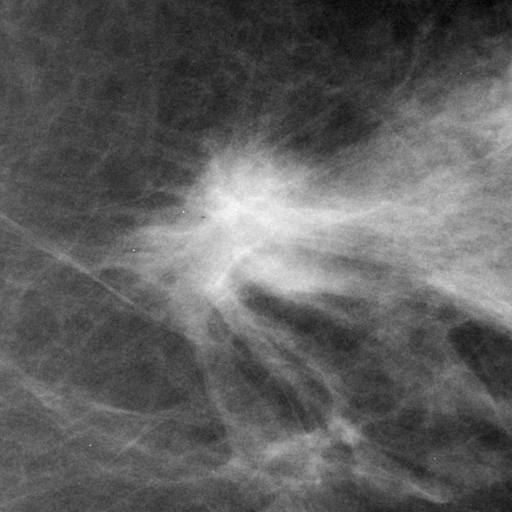
\includegraphics[width=\qtrcol]{\figpath/ipmi/mass046} &
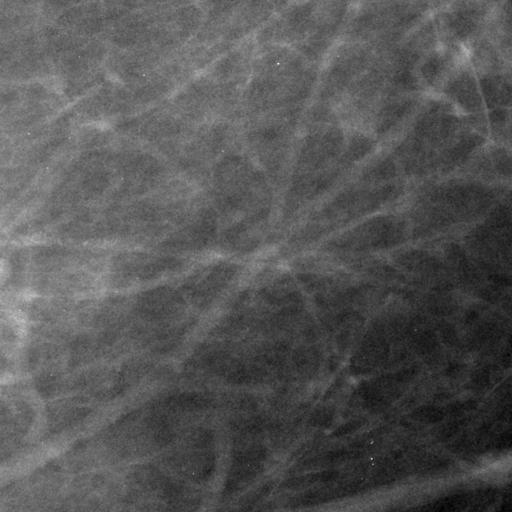
\includegraphics[width=\qtrcol]{\figpath/ipmi/norm068} \\
(a) & (b) \\
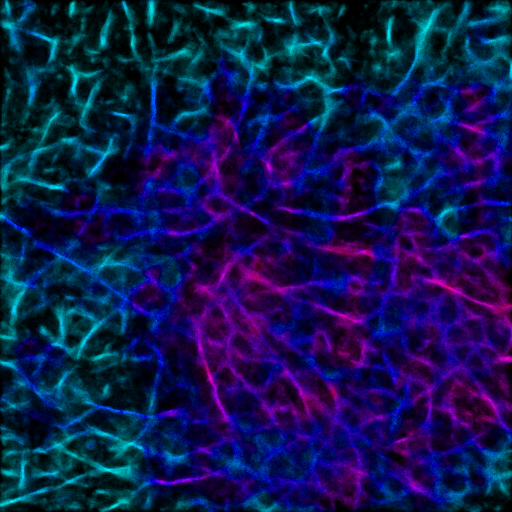
\includegraphics[width=\qtrcol]{\figpath/ipmi/spic_prob_mass046_a} &
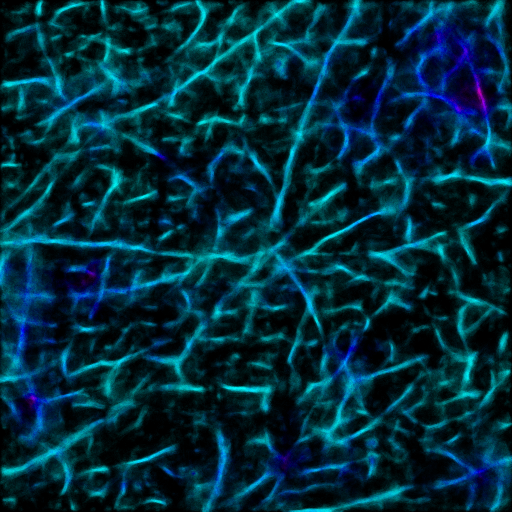
\includegraphics[width=\qtrcol]{\figpath/ipmi/spic_prob_norm068_a} \\
(c) & (d)
\end{tabular}
%
\caption{Regions depicting (a) malignant and (b) normal tissue. The corresponding spicule classification results are depicted in (c,d) using hue to indicate abnormality -- ranging from cyan (normal) to pink (spicule) -- and intensity to indicate the line detection output from the DT-CWT method.}
\label{f:mammogram_examples}
\end{figure}


\begin{figure}
\centering
\begin{tabular}{c c c c}
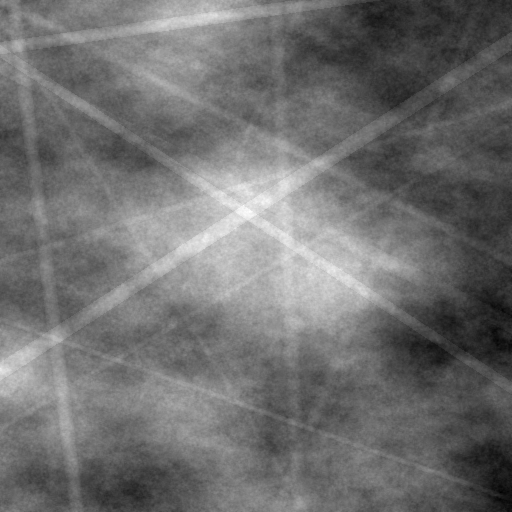
\includegraphics[width=\qtrcol]{\figpath/ipmi/line512_003} &
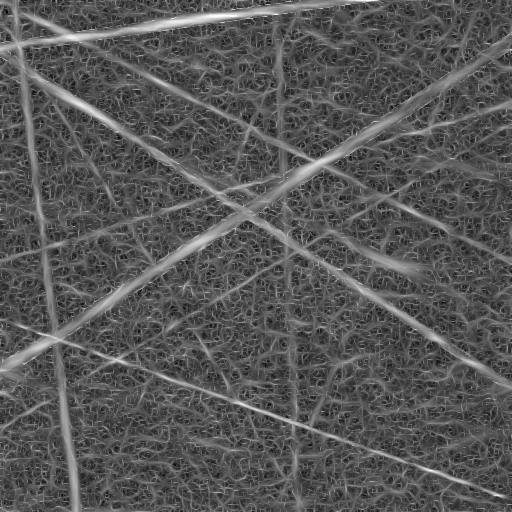
\includegraphics[width=\qtrcol]{\figpath/ipmi/line512_003_lines} &
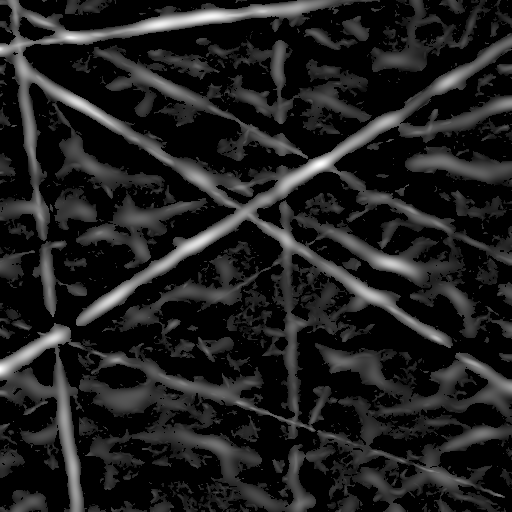
\includegraphics[width=\qtrcol]{\figpath/ipmi/line512_003_gaussian} &
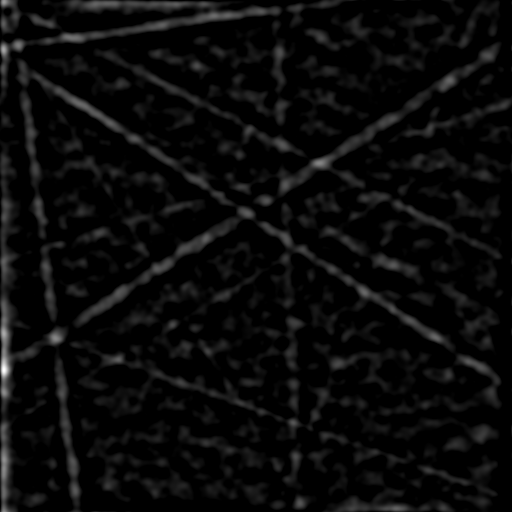
\includegraphics[width=\qtrcol]{\figpath/ipmi/line512_003_monogenic} \\
(a) & (b) & (c) & (d) \\
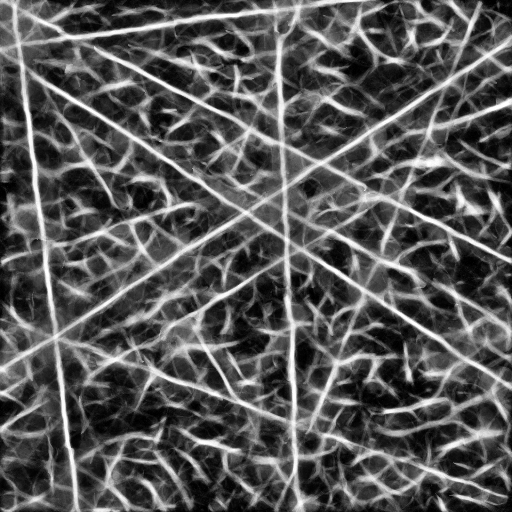
\includegraphics[width=\qtrcol]{\figpath/ipmi/line512_003_rf_191905} &
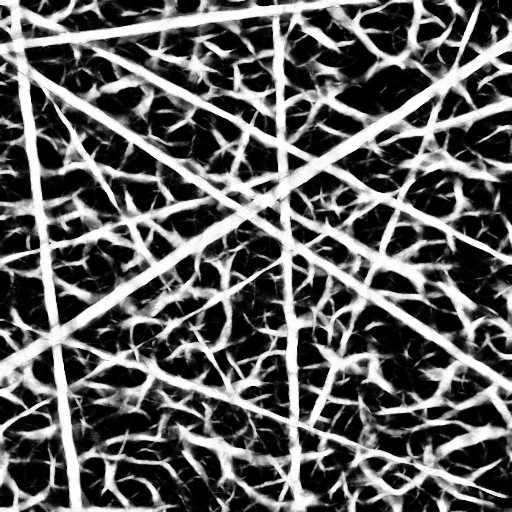
\includegraphics[width=\qtrcol]{\figpath/ipmi/line512_003_rf_191961} &
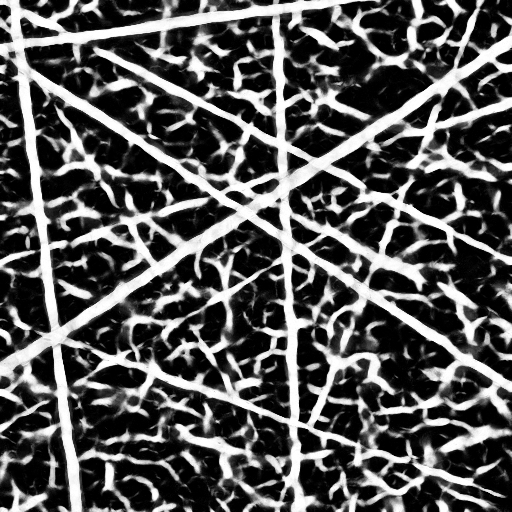
\includegraphics[width=\qtrcol]{\figpath/ipmi/line512_003_rf_233141} &
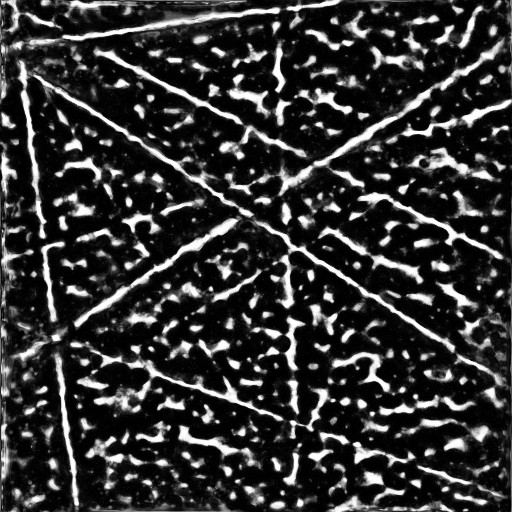
\includegraphics[width=\qtrcol]{\figpath/ipmi/line512_003_rf_191960} \\
(e) & (f) & (g) & (h)
\end{tabular}
%
\caption{Synthetic test image and corresponding filter responses: (a) original image; (b) Linop; (c) Gaussian; (d) Monogenic; (e) DT-CWT/RF; (f) Linop/RF; (g) Gaussian/RF; (h) Monogenic/RF.}
\label{f:synthetic_responses}
\end{figure}


\begin{figure}
\centering
\begin{tabular}{c c c c}
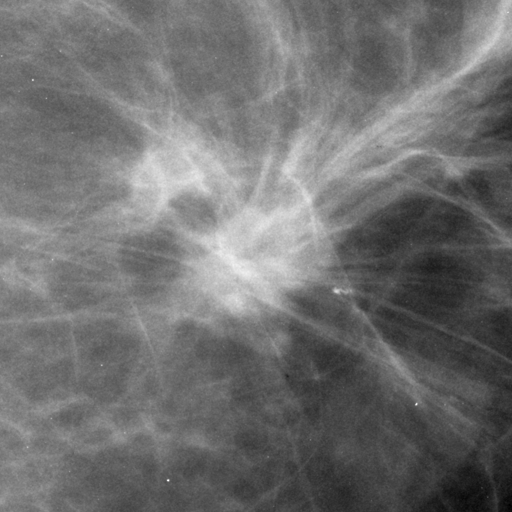
\includegraphics[width=\qtrcol]{\figpath/ipmi/mass028} &
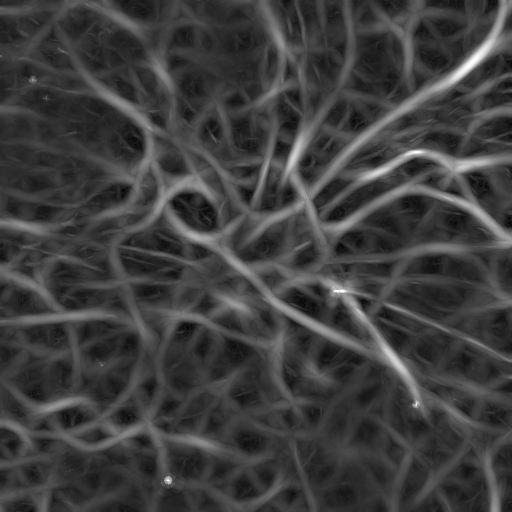
\includegraphics[width=\qtrcol]{\figpath/ipmi/mass028_linop} &
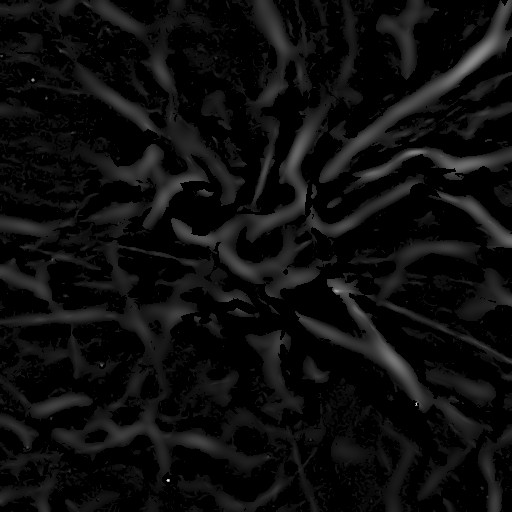
\includegraphics[width=\qtrcol]{\figpath/ipmi/mass028_gaussian} &
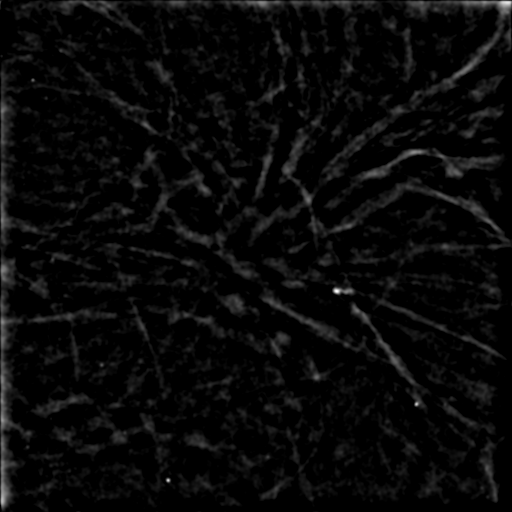
\includegraphics[width=\qtrcol]{\figpath/ipmi/mass028_monogenic} \\
(a) & (b) & (c) & (d) \\
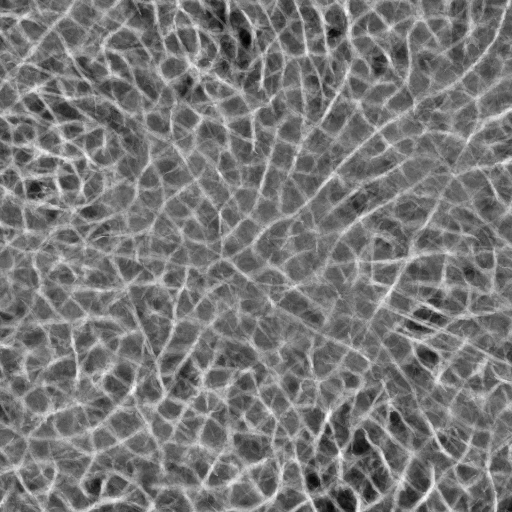
\includegraphics[width=\qtrcol]{\figpath/ipmi/mass028_dt} &
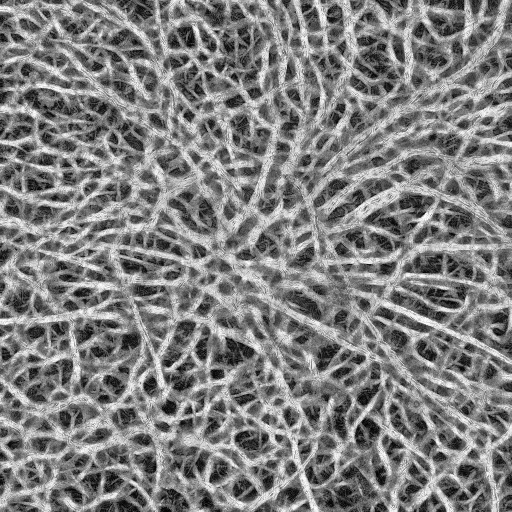
\includegraphics[width=\qtrcol]{\figpath/ipmi/mass028_rf_linop_w1l5} &
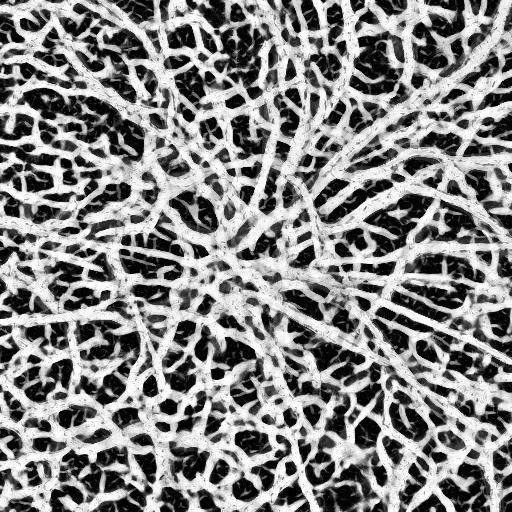
\includegraphics[width=\qtrcol]{\figpath/ipmi/mass028_rf_gaussian} &
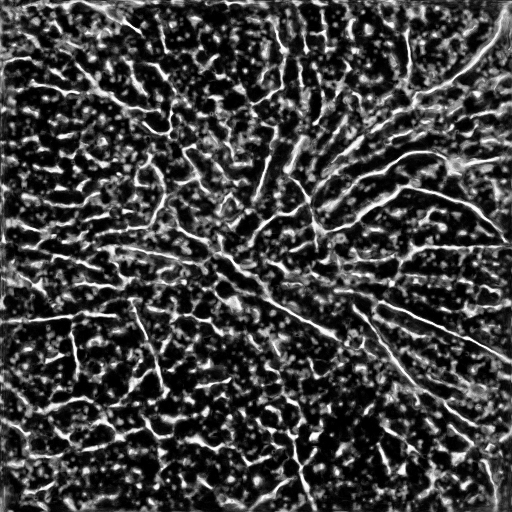
\includegraphics[width=\qtrcol]{\figpath/ipmi/mass028_rf_monogenic_w3l4} \\
(e) & (f) & (g) & (h)
\end{tabular}
%
\caption{Mammogram region containing malignant spiculated mass and corresponding filter responses: (a) original image; (b) Linop; (c) Gaussian; (d) Monogenic; (e) DT-CWT/RF; (f) Linop/RF; (g) Gaussian/RF; (h) Monogenic/RF.}
\label{f:real_responses}
\end{figure}


\begin{figure}
\centering
\begin{tabular}{c c c}
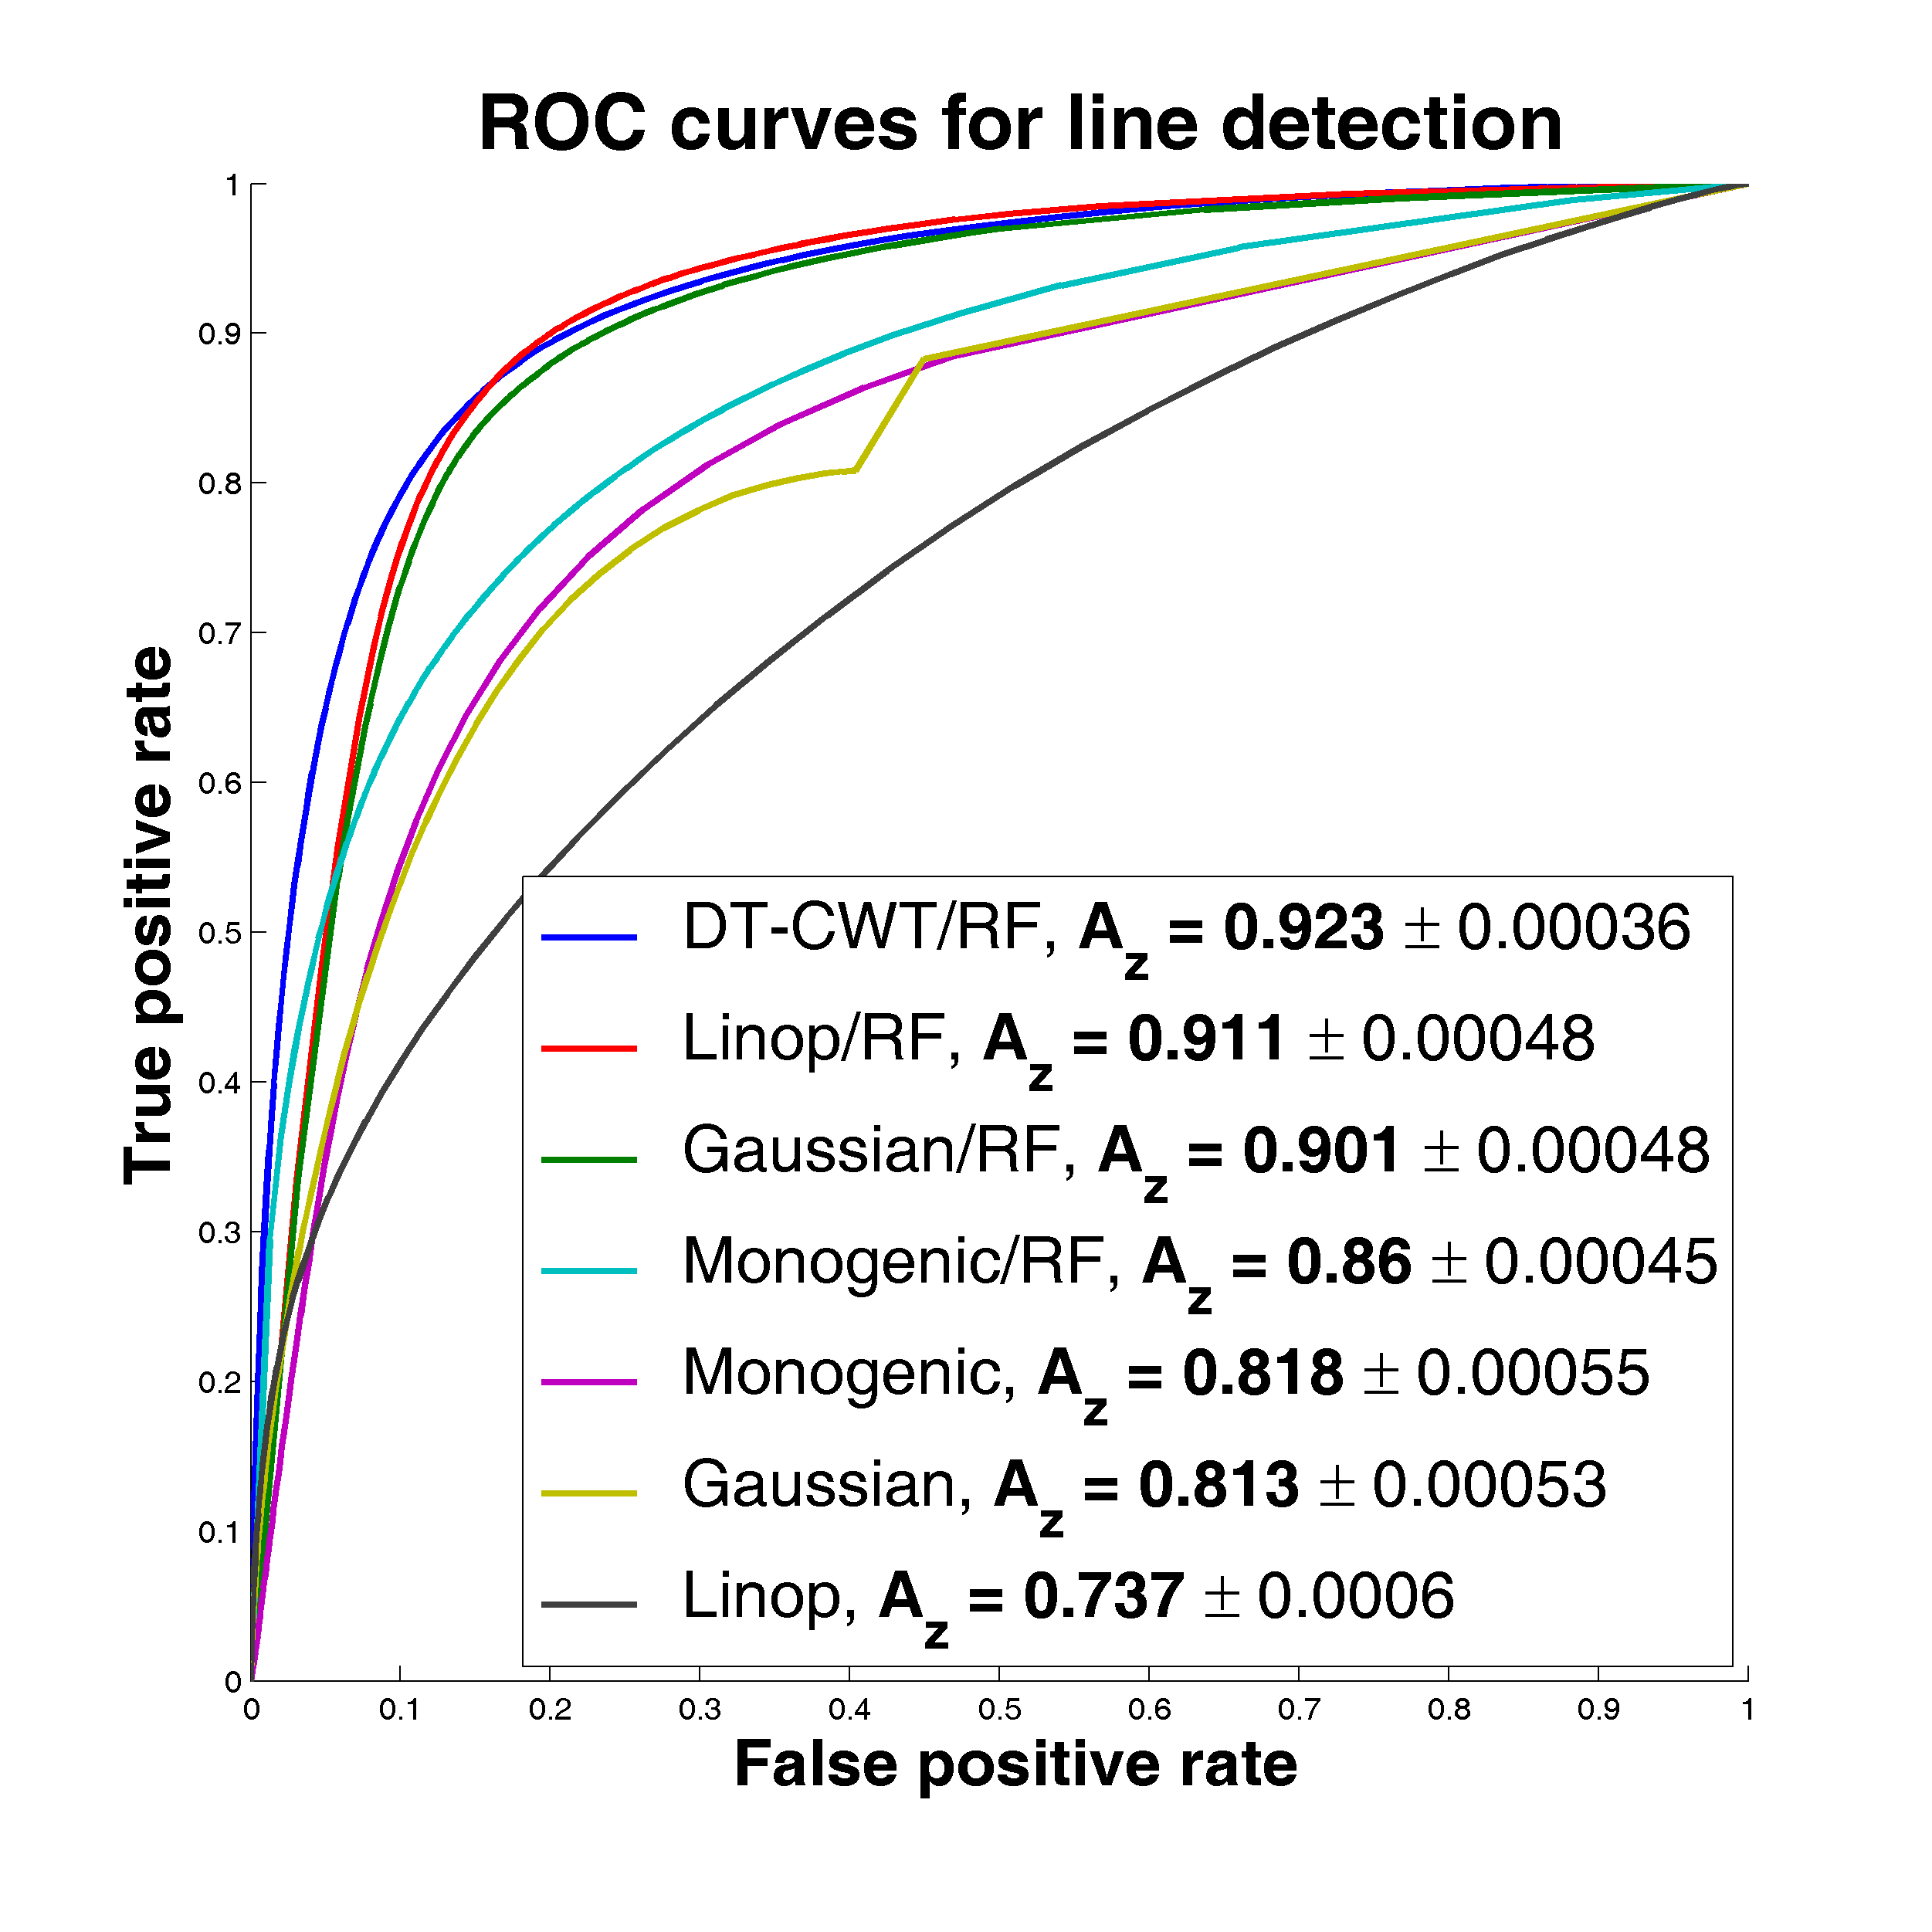
\includegraphics[width=0.33\columnwidth]{\figpath/ipmi/line_detection_roc} &
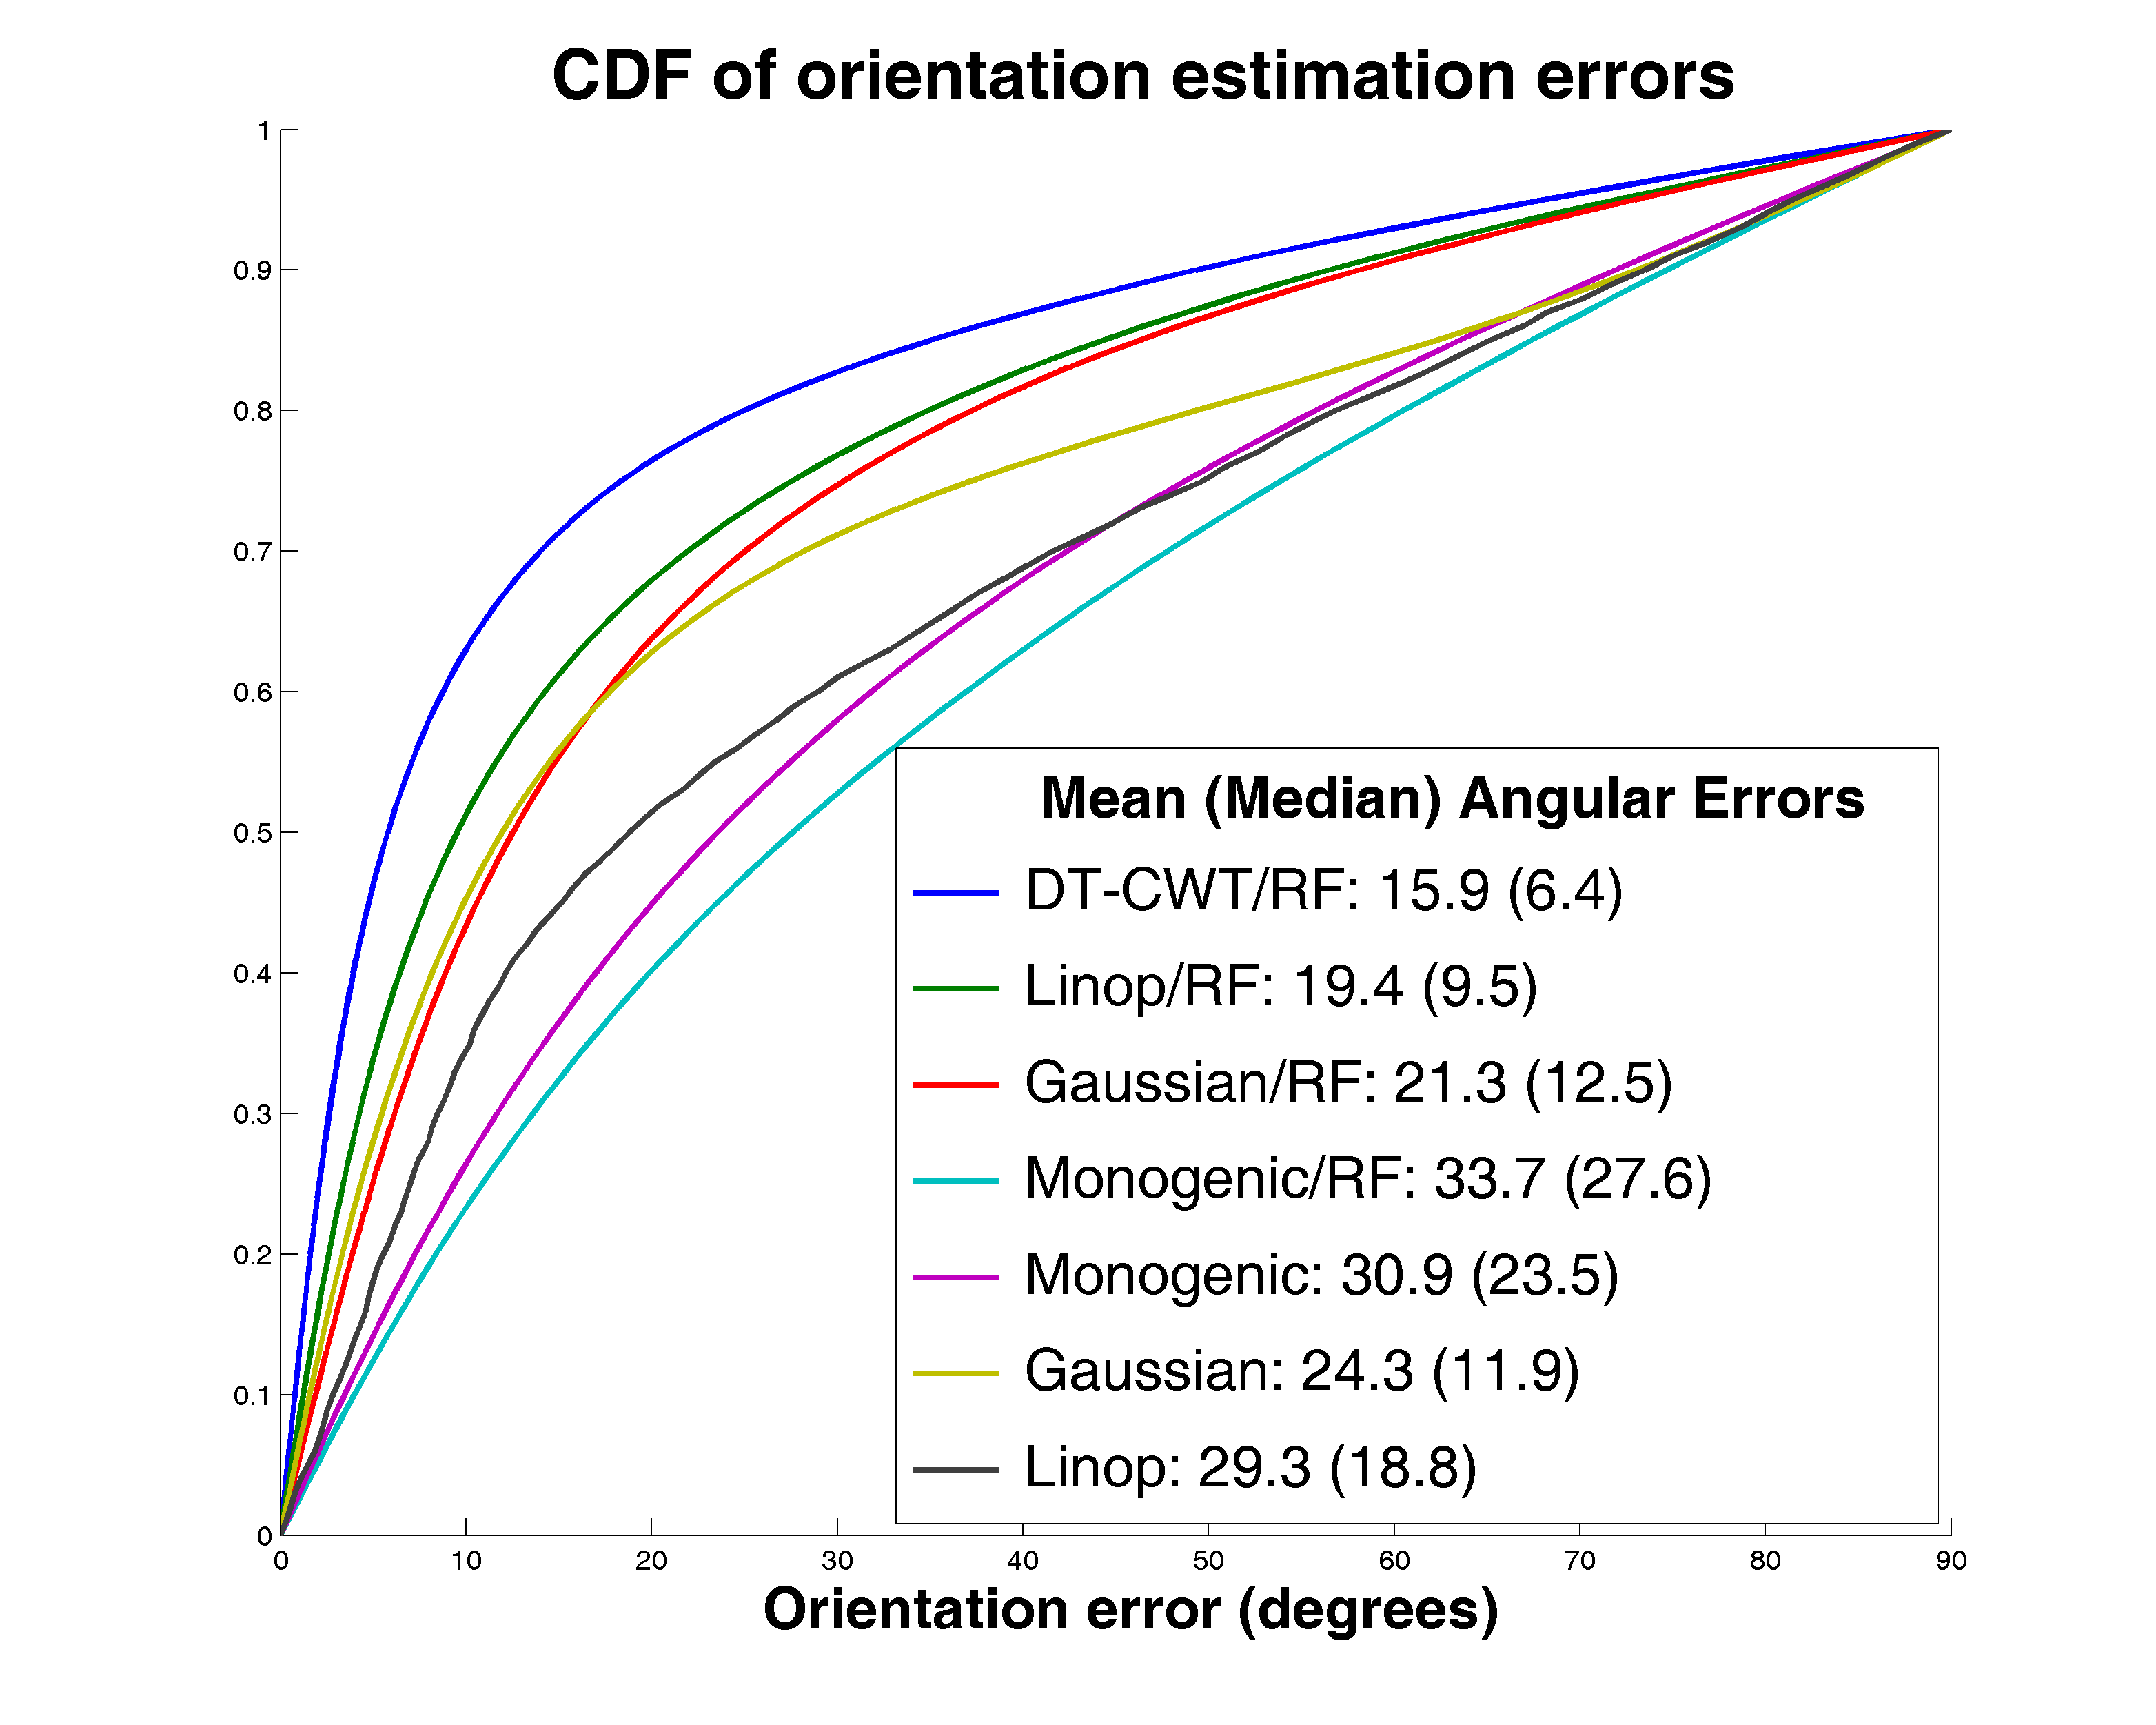
\includegraphics[width=0.33\columnwidth]{\figpath/ipmi/orientation_estimation_cdf} &
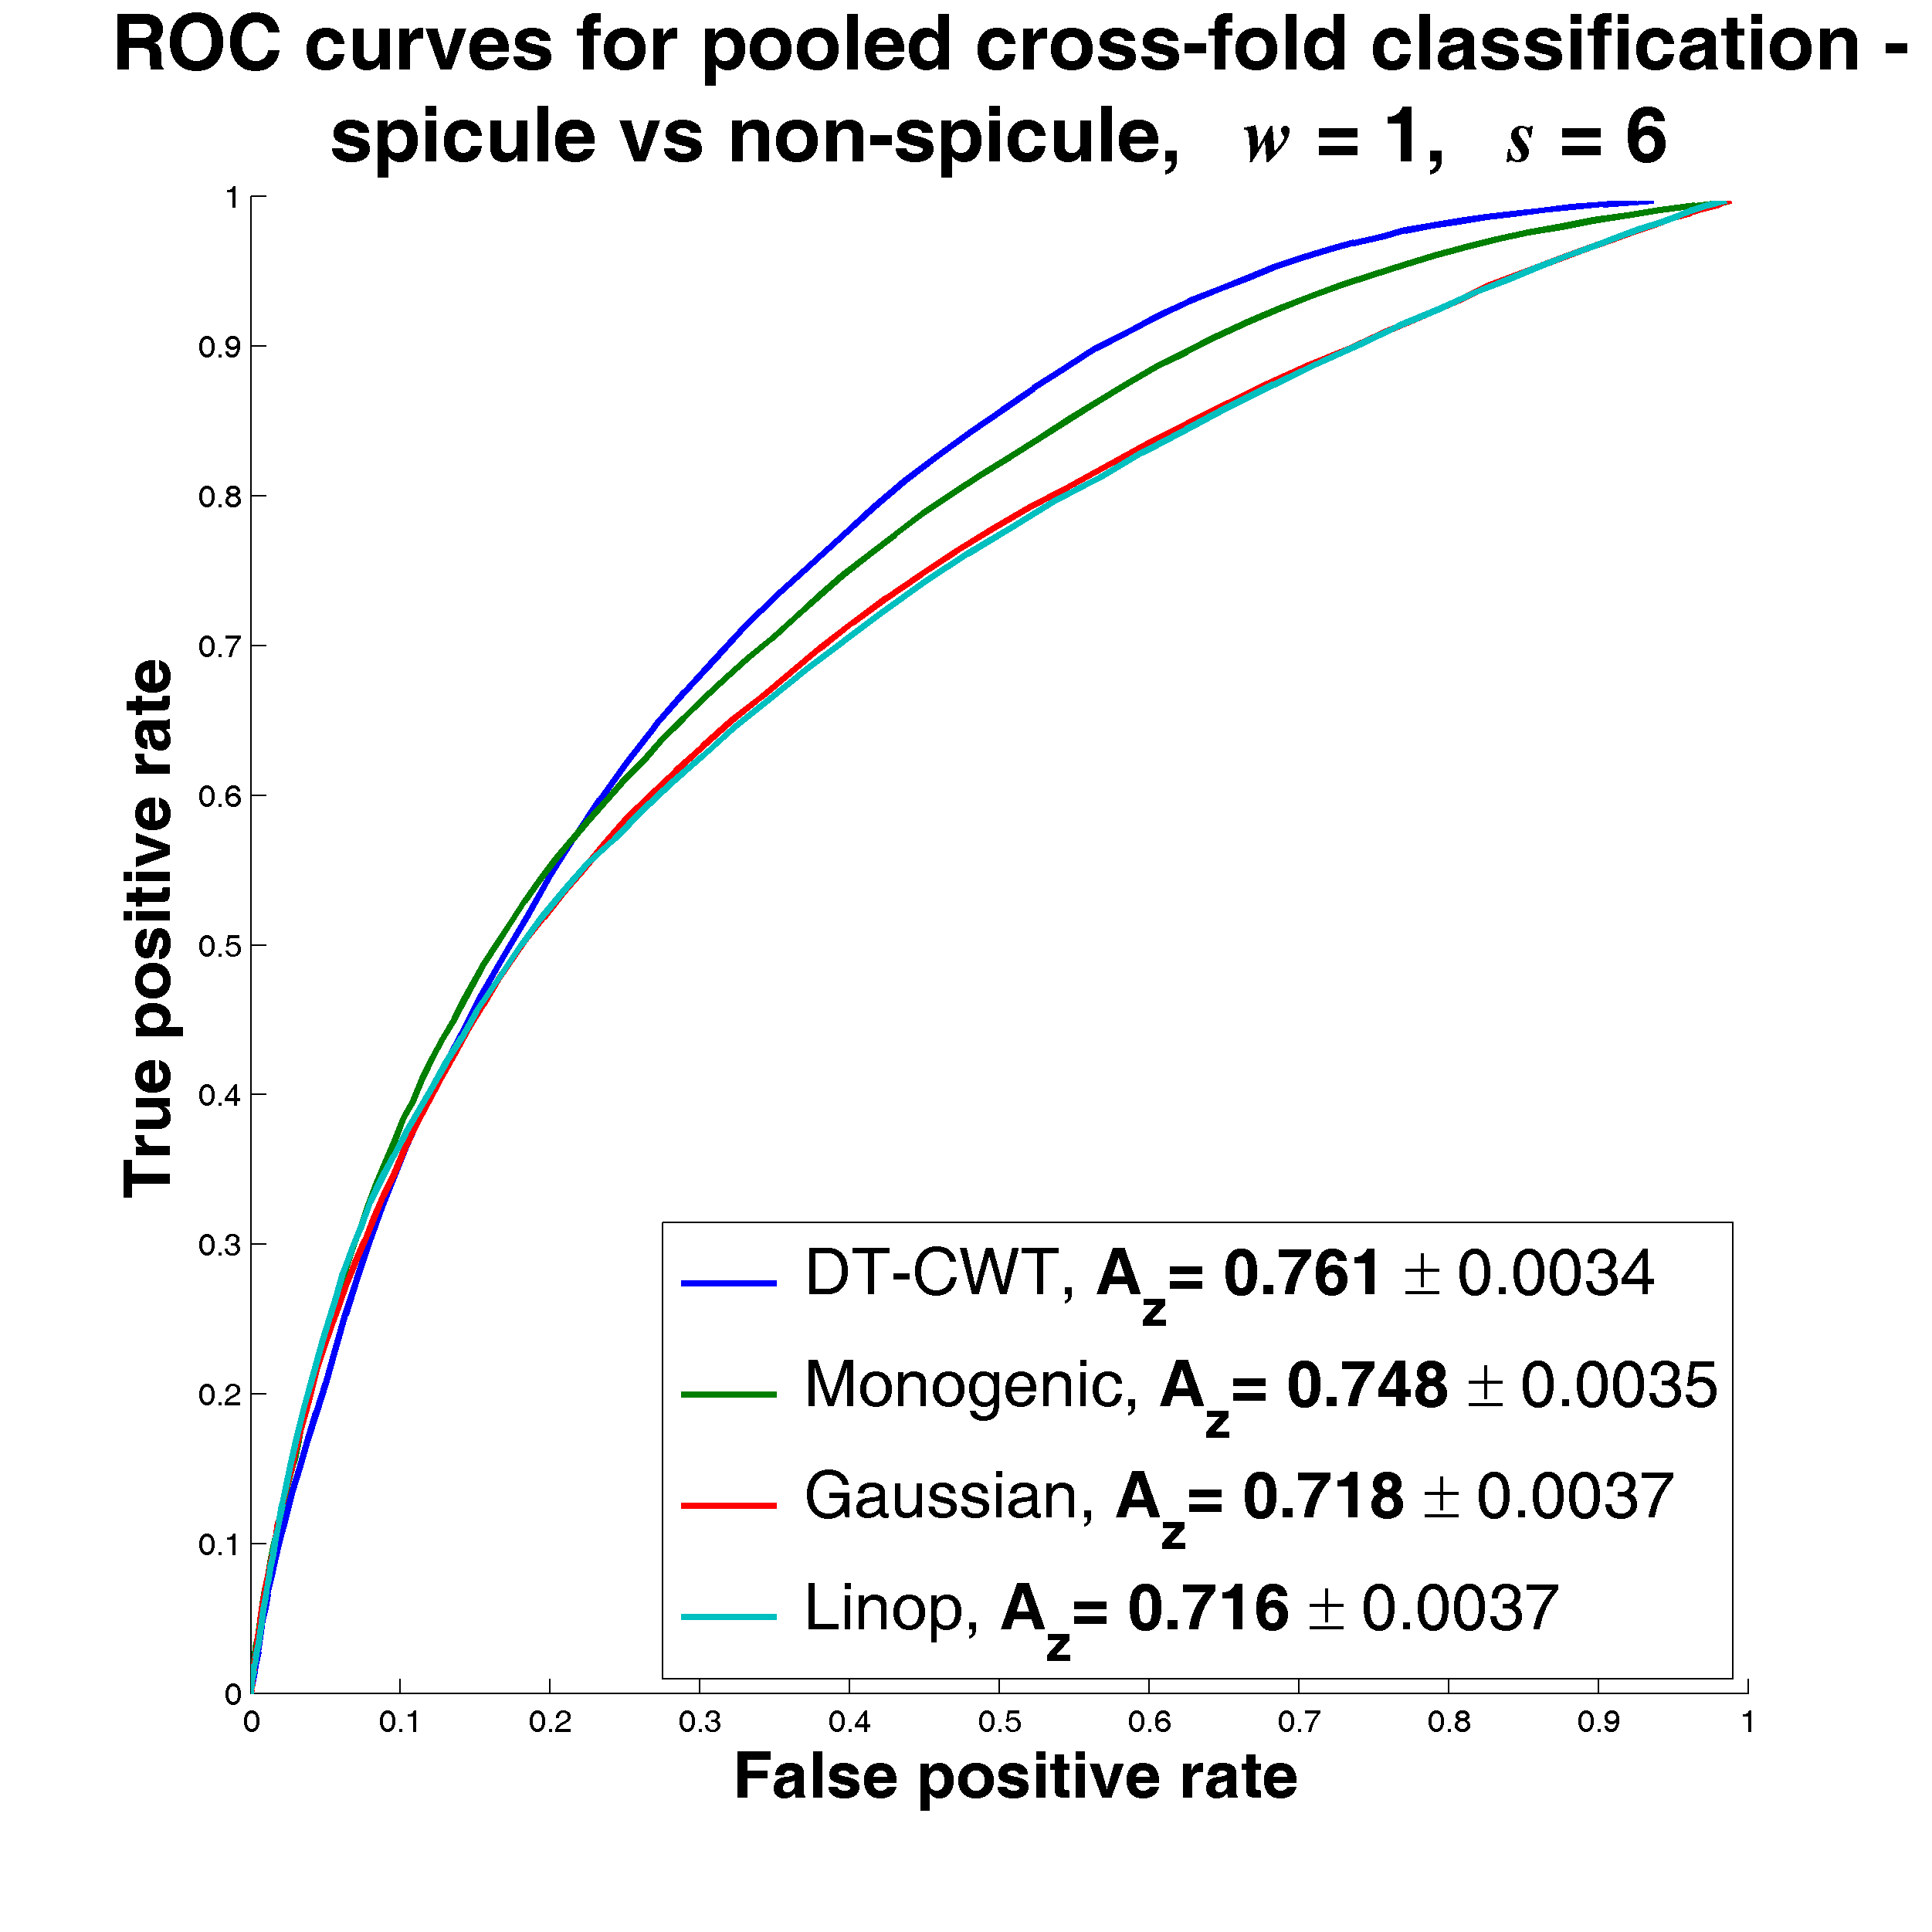
\includegraphics[width=0.33\columnwidth]{\figpath/ipmi/rf_spic_1_6}
\end{tabular}
%
\caption{Receiver operating characteristic (ROC) curves for different curvilinear structure detection methods; centre: Cumulative distribution functions (CDF) of errors in orientation estimation for the different methods; right: ROC curves for spicule classification.}
\label{f:detection_roc}
\end{figure}


\begin{table}
\centering
\caption{Line detection and orientation computation results. For every algorithm, we present the area under the ROC curve ($A_z$), the sensitivity at 90\% specificity, and the mean absolute error of the orientation estimate.}
\label{t:line_detection}
%
\begin{tabular}{l c c c}
Algorithm	
		& $A_z$							& Sens. \@ 90\% spec. & MAE \\
\hline
DT-CWT/RF ($w$ = 1, $s$ = 5)												
		& 0.923$\pm$0.00036	& 0.792 							& 15.88 \\
Linop/RF ($w$ = 1, $s$ = 5, 8 orientations)				
		& 0.911$\pm$0.00048	& 0.757								& 19.35 \\
Gaussian/RF ($w$ = 1, $s$ = 4, $\sigma_{min}$ = 1)
		& 0.901$\pm$0.00048	& 0.731								& 21.37 \\
Monogenic/RF ($w$ = 1, $s$ = 4, $\lambda$ = 4)
		& 0.868$\pm$0.00045	& 0.643								& 33.73 \\
Monogenic ($s$ = 3, $\lambda$ = 4)									
		& 0.818$\pm$0.00055	& 0.547								& 30.86 \\
Gaussian ($s$ = 4, $\sigma_{min}$ = 1)							
		& 0.813$\pm$0.00053	& 0.533								& 24.27 \\
Linop ($s$ = 5, 8 orientations)										
		& 0.737$\pm$0.00060	& 0.413								& 29.32 \\
\end{tabular}
\end{table}


\begin{table}
\caption{Results for spicule classification. For every algorithm, we show the area under the ROC curve ($A_z$)}
\label{t:spicule_classification}
%
\begin{tabular}{l c}
Algorithm
		& ROC $A_z$ \\
\hline
DT-CWT/RF ($w$ = 1, $s$ = 6, all orientations)
		& 0.761$\pm$0.0034 \\
Monogenic/RF ($w$ = 1, $s$ = 5, 8 orientations)
		& 0.748$\pm$0.0035 \\
Gaussian/RF ($w$ = 1, $s$ = 5, $\sigma_{min}$ = 1)
		& 0.718$\pm$0.0037 \\
Linop/RF ($w$ = 1, $s$ = 5, $\lambda$ = 4)
		& 0.716$\pm$0.0037 \\
\end{tabular}
\end{table}

%\chapter{Classifying Linear Structure}

Classification is of interest when it is important to distinguish between subtly different structures which may be present within the same image - for example, rivers and roads

The learning approach described above can also be used to differentiate between different kinds of curvilinear structure. The hypothesis is that the cross-sectional intensity profiles of structures differ in systematic ways between types of mammographic structure (as suggested by Zwiggelaar et al~\cite{Zwiggelaar_etal_TMI04}), and that profile shape is effectively captured by the DT-CWT coefficients - particularly in the phase components. In the experiments described below we concentrated on the task of distinguishing between spicules, which are a sign of malignancy, and other curvilinear structures. Although it was not realistic to create a training set of mammogram images with all spicules annotated, we were able to obtain expert annotations of a reasonably large number of spicules in a set of mammogram patches containing malignant tumours (see section 5.1 for details). These annotations were used to select pixels for the positive training set. To create a balanced training set we sampled feature vectors from the same number of pixels in a set of normal mammogram patches, such that the distribution of curvilinear structure probabilities was the same as for the spicule training set. Using this balanced training set, we built a random forest classifier to perform spicule/non-spicule classification.

The literature on classifying curvilinear structures in mammograms is much more limited. We are aware of the work of Zwiggelaar et al~\cite{Zwiggelaar_etal_TMI04}, which demonstrated the feasibility of distinguishing between different types of structure using cross-sectional profiles obtained from manually annotated curvilinear structures, but did not obtain very satisfactory results when the method was fully automated.  We recently reported preliminary classification (but not detection) results using our current approach~\cite{Chen_etal_IWDM10}.


\section{Experimental Evaluation}
We have conducted a systematic evaluation of the performance of our method for curvilinear structure detection and classification, using both synthetic and real mammogram data, comparing seven competing approaches:

\begin{itemize}
\item DT-CWT/RF: the method described in this paper.
\item Monogenic: the monogenic-signal phase congruency approach~\cite{Wai_etal_MICCAI04}.
\item Linop: the Line operator~\cite{Dixon_Taylor_IPC79,Parr_etal_SPIE97}.
\item	Gaussian: the directional Gaussian 2nd derivatives~\cite{Karssemeijer_teBrake_TMI96}.
\item	Monogenic/RF: the raw responses used in Monogenic, combined using RF classification.
\item	Linop/RF: the raw responses used in Linop, combined using RF classification.
\item Gaussian/RF: the raw responses used in Gaussian, combined using RF classification.
\end{itemize}

Monogenic, Linop and Gaussian are representative of the current state of the art in line detection. Monogenic/RF, Linop/RF and Gaussian/RF are natural variants, in which the intermediate multiscale responses previously used to construct the detection outputs are instead combined to given feature representation at each pixel that can subsequently classified using a random forest. These learning variants were developed for two reasons: firstly, when analyzing quantitative results for detection performance, they allow us to decouple the effect of random forest learning from the effect due to the type of representation used. Secondly, unlike their original variants, Monogenic/RF, Linop/RF and Gaussian/RF can be used in the spicule classification experiment described in 5.3.

In what follows, we present both qualitative and quantitative results for detection and classification for each method outlined above. 

\subsection{Data}
\paragraph{Synthetic Data.} We used two sets of synthetic images containing curvilinear structures, with known ground truth, to train and test curvilinear structure detection. We randomly extracted 4 \by 4 cm (512 \by 512 pixel) mammographic backgrounds with 256 grey-levels 72 (30) normal mammograms for the training (test) set, resulting in 10460 training patches and 4903 test patches, from which naturally occurring linear structures were filtered out. Lines were added to these backgrounds, with parameters drawn from the following distributions: orientation [0, ?] uniform; width [4, 16] pixels uniform; peak intensity [1,255] grey-levels (relative to images scaled 0 - 255) from an exponential distribution with half-width 4 grey-levels; profile shape ? determined by the equation ? = ? + (1- ?) sinx for offsets x  (0,?), where the 'squareness' parameter ? determines how close the shape is to a pure half-cycle sin or a rectangle and is drawn uniformly from [0,1]. The range of widths, distribution of contrasts (with low contrast lines much more likely than high contrast lines) and variability in profile shape were chosen to mimic what is found in real mammograms.

During training, backgrounds were randomly sampled from the 10460 training patches and a single line was added to the centre of the patch. These images were produced 'on-the-fly' during each tree-building step of random forest construction as described in section 5.2 and no permanent set was maintained.

For testing, 100 backgrounds were randomly selected from the test patches. To each, multiple lines were added sequentially, with the number and position of lines varying randomly. An example of a synthetic image is shown in Fig 1(a).

Note that all synthetic lines used were straight lines. We conducted experiments explicitly using curved structures, however as there was no performance difference between training on curved or straight lines when detecting curved lines, it was decided that including curves was unnecessary.

\subsection{Real Mammogram Data}
We used real mammogram patches to illustrate qualitative results for curvilinear structure detection and to train and test spicule/non-spicule classification. Data were taken from a sequential set of 84 abnormal mammograms with biopsy-proven malignancy, drawn from a screening population (Nightingale Breast Centre, South Manchester University Hospitals Trust, UK), and from a set of 89 normal mammograms of the contralateral breasts of the same individuals (where disease was radiologically confirmed to be confined to one breast). All mammograms were digitised to a resolution of 90�m, using a Vidar CADPRO scanner. A 4x4 cm patch was extracted around each abnormality, and a similar patch was sampled randomly from each of the normal mammograms; examples are shown in \ref{f:} 4. For each abnormal patch an expert radiologist manually annotated some (though not necessarily all) of the spicules associated with the abnormality, resulting in a total of 555 spicule annotations. The expert spicule annotations for the abnormal images were used as a basis for selecting spicule pixels, though they were not sufficiently accurate to be used directly. To refine the annotations, we initialised a snake~\cite{Kass_etal_IJCV88} using each original annotation, and iterated it to convergence, using evidence from the linear structure probability image. We note that a similar technique has recently been published in detail by Muralidhar et al~\cite{Muralidhar_etal_TMI10}. As a result, the 555 refined spicule annotations identified a set of 36,514 spicule pixels. As outlined in section 4, we sampled the same number of pixels from the normal images, such that the detection probability distributions for the spicule and non-spicule samples were the same.

\subsection{Spicule Classification}
The four learning-based methods were also applied to the problem of spicule/non-spicule classification. Feature vectors were formed as above, and random forest classifiers were trained using balanced spicule/non-spicule training data, as outlined in section 4. To make effective use of the available data, we used a 10-fold cross-validation design. The set of normal and abnormal regions were divided into 10 groups so that the total number of normal and spicule pixels in each group were as close as possible to a 10th of the total and no two views from the same case were included in different groups. The samples in each group were then classified using a random forest trained on the samples from the remaining 9 groups. The classification results from each group were pooled to generate an unbiased class probability for each sampled pixel. These probabilities were used to compute an ROC curve for each training regime, and the area under the curve (Az) was computed and used as a measure of classification performance. The ROC curves and Az values for the three methods are shown in \ref{f:} 2 and \ref{t:} 2. These results demonstrate a clear advantage for DT-CWT/RF. As might be expected, because the Linop and Gaussian representations do not really capture profile shape, they perform significantly worse that the two representations that include phase.

In addition to computing a class vote for spicule membership at only those pixels in the selected training sets, the forests we have constructed can be used to compute results for whole region in each cross-fold group. Typical qualitative DT-CWT/RF results for a normal and abnormal region are shown in \ref{f:} 4. In the left column, the original regions are shown. The spiculations of the mass are clear and well defined, particularly to the south-east of the central mass. In the normal region, there are a set of structures that intersect in an approximate radial pattern that may trigger a feature detector erroneously. In the right column, the predicted spicule class membership is shown as hue varying from cyan (normal) to pink (spicule), modulated by the output of the DT-CWT/RF detection method. Note how the linear structures in the region of the mass are deemed highly likely to be spicules, whilst those in the normal region are not. This shows excellent promise as a means of providing a relevance measure to methods for abnormality detection.

\section{Discussion}
We have presented a discriminative learning-based approach to the detection and classification of curvilinear structures, based on a combination of DT-CWT representation of local structure and random forest classification. We have applied the method to the challenging problem of detecting and estimating the orientation of curvilinear structures in mammograms and distinguishing between normal and abnormal structures. The results of our experimental evaluation are extremely encouraging, and represent a significant improvement over the current state of the art. 

We have also introduced learning-based variants of three existing methods, demonstrating that whilst learning accounts for a significant part of this improvement, the choice of representation is also important and will have a different effect on performance depending on the task in hand. For example, constructing a representation based on the raw responses to Linop filters produces features that are excellent for estimating structure orientation but provide less information for determining structure shape and thus type. Conversely, features formed from the monogenic signal are good at determining structure type - most likely because of the inclusion of the phase measure - whilst they perform relatively poorly at detection and orientation estimation. For these reasons, it seems fair to conclude that the DT-CWT provides the best all round representation. It produced the strongest performance for all three tasks (curvilinear structure detection, orientation estimation and spicule classification). Moreover, as discussed in section 5.2, of all the methods, the DT-CWT incurs the least overhead when working with full-size real images that require block-wise classification/regression. For example, initial tests show that the structure detection and orientation regression can be performed on a full-size (~3000 x 2400 pixels) mammogram in ~1hr 30mins.

Our next goal is to show that improving the individual steps of curvilinear structure and orientation estimation result in a subsequent improvement for a high level task such as detecting patterns of spiculations indicative of disease. Moreover we hope to show that classification into structure type can further aid such tasks by focusing only (or at least more) on those structures most likely to be associated with disease.

%\chapter{Line Properties}

\section{Introduction}
\label{s:introduction}
Curvilinear structures are important in many applications of computer vision, including aerial image analysis (roads, rivers, railways), fingerprint analysis (ridges) and medical image analysis (blood vessels, ducts). As a result, there is an extensive literature on detecting such structure~\cite{Papari_Petkov_IVC11}. The literature on estimating the local orientation of curvilinear structure is more limited though the problem is equally important, for example as a basis for non-maximal suppression (centre-line detection) and for characterising properties such as tortuosity (\eg~of blood vessels).

In mammography, malignant lesions often exhibit linear structures (known as spicules) that form a radial pattern around the central mass. Detecting linear structures and determining their orientation~\cite{Zwiggelaar_etal_MIA99,Zwiggelaar_etal_TMI04} can therefore indicate points where they converge and thus whether a mass or architectural distortion is present~\cite{Karssemeijer_teBrake_TMI96,Rangayyan_Ayres_MBEC06}. In other medical applications such as retinography (\fref{f:retinography}), the rate of change of orientation (\ie~tortuosity) of blood vessels can serve as a diagnostic indicator of vascular disease~\cite{Hart_etal_IJMI99}; though studies have shown that vessels can be detected and segmented~\cite{Staal_etal_TMI04,Ricci_Perfetti_TMI07,Dabbah_etal_MICCAI10}, few have addressed the problem of measuring their orientation and quantifying tortuosity.

Similarly, automatic fingerprint analysis typically begins by computing the orientation at each pixel via gradient-based filtering, often followed by some smoothing over a local patch~\cite{Bazen_Gerez_TPAMI02,Mei_etal_IVC09}. This orientation field is often parameterized -- via `phase portraits'~\cite{Li_etal_PR06} or polynomial approximation~\cite{Gu_etal_PR04}, for example -- to capture and interpret the underlying properties of the fingerprint such as its `singular points' where the orientation is no longer defined (\eg~at a delta or the centre of a whorl). Though smoothing orientation estimates at a local patch have been the subject of several investigations~\cite{Kass_Witkin_CVGIP87,Rao_Jain_TPAMI92,Perona_TIP98}, we deal only with the initial step of estimating orientation at every pixel.

In this paper we revisit the problem of orientation estimation, reviewing the basic theory, extending the state-of-the-art, and providing the results of extensive evaluation using both real and realistic synthetic images. The first step in estimating orientation usually involves applying a set of linear filters to the image, generally at multiple scales and orientations. As we will show later, the choice of filter-bank has a significant influence on both computational efficiency, and estimation accuracy. Our contribution is to explore the similarities and differences between different approaches, and provide empirical evidence of which work best in practice.

Given a set of filter-bank outputs, the second step in estimating orientation is to combine them in some way. There are two basic approaches: to find the scale at which the total magnitude of response is greatest, and combine the different filter responses at that scale analytically~\cite{Karssemeijer_teBrake_TMI96,Mei_etal_IVC09}; or to use a regression learning approach to combine the filter responses across all scales and orientations~\cite{Berks_etal_IPMI11}. Our contribution is to explore the technical details of orientation regression and provide a comprehensive evaluation of different combinations of filter-bank and analytic/regression methods. Overall we show that an approach based on combining dual-tree complex wavelet filtering with random forest regression achieves significantly better results than any of the other state-of-the-art approaches tested.

\begin{figure}[t]
\centering
\begin{tabular}{c c c}
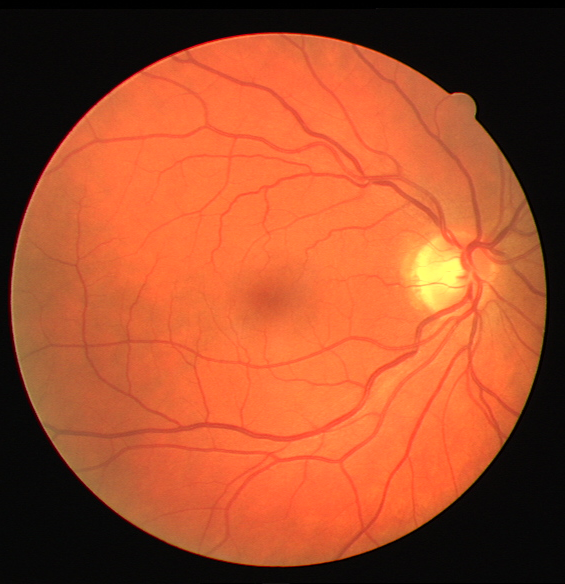
\includegraphics[width=0.3\columnwidth]{\figpath/retina/02_test} &
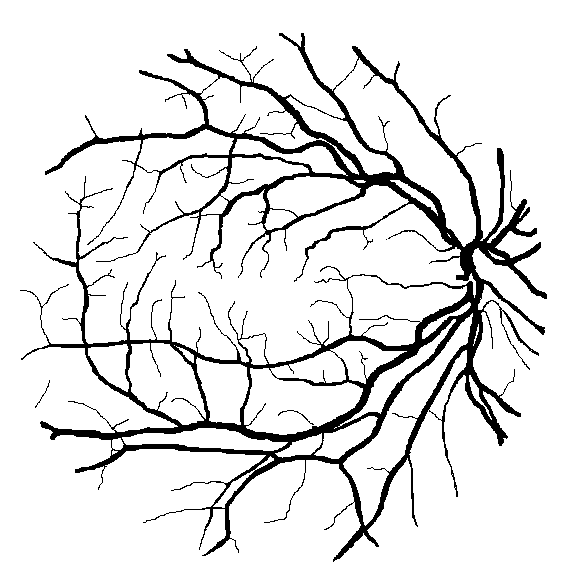
\includegraphics[width=0.3\columnwidth]{\figpath/retina/02_manual1} &
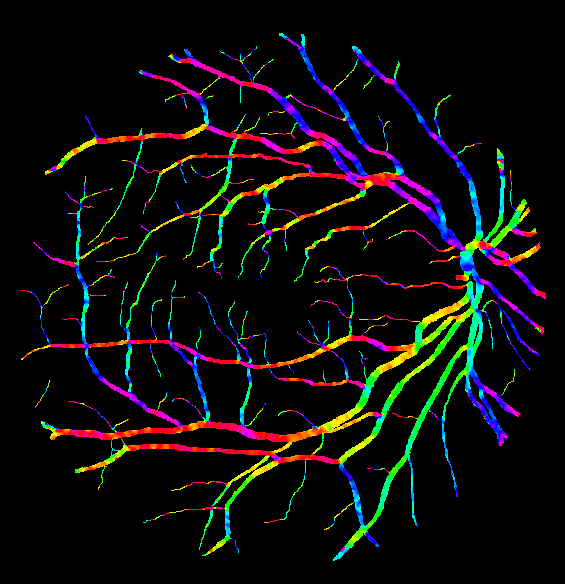
\includegraphics[width=0.3\columnwidth]{\figpath/retina/002_orientation_masked} \\
%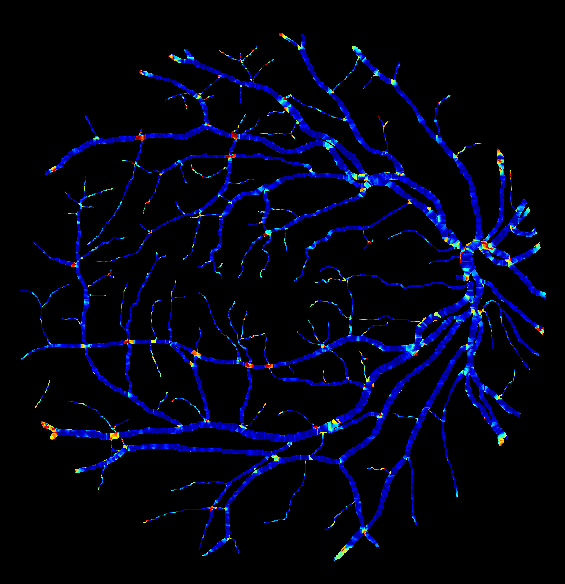
\includegraphics[height=0.15\textheight]{\figpath/retina/002_abs_error} \\
(a) & (b) & (c) \\
\end{tabular}
%
\caption{Estimating orientation in retinography: %
(a) input image; %
(b) ground truth mask indicating pixels belonging to a vessel; %
(c) orientation (indicated by colour) estimated using linear regression over \dtcwt~features. The mask was not used to estimate orientation. %
%(c) magnitude of error (note the regions of high error at points of bifurcation.)
}
\label{f:retinography}
\end{figure}




\section{Estimating Orientation via Machine Learning}
\label{s:learning}


\section{Experiments}
\label{s:expts}
In our first set of experiments, we present a quantitative evaluation of the three regressors on real retinography images and mammogram-like data for which we have ground truth. We also present qualitative results on some real mammography images and fingerprint images for which ground truth was not available.


\subsection{Real Retinographic Images}
\label{s:expts_retinography}
The publicly available DRIVE dataset~\cite{Staal_etal_TMI04} contains 40 full colour retinogram images (\fref{f:retinography}a) of $565{\times}584$ pixels, split into training (images 21-40) and test (images 01-20) sets. A hand-labelled mask that indicates vessel pixels (\fref{f:retinography}b) is also available for every image, enabling us to skeletonize the mask and approximate ground truth, $\theta_{gt}$, from the skeleton for every labelled pixel.\comment{It is questionable how well this constitutes ground truth}

For training, we first transform all images to monochrome via a weighted sum of the three RGB channels (though using only the green channel is also popular). We then selected 200\,000 vessel pixels randomly over the training set and computed filter responses to the second derivative filters (\fref{f:filters}e-f), Haar-like filters (\fref{f:filters}g-h) and the \dtcwt~for every selected pixel. We used the resulting 200\,000 feature vectors and their corresponding target orientations to train each of the three regressors.

During testing, we applied each regressor in turn to estimate the orientation, $\theta_{est}$, at every pixel for every test image and computed the orientation error with respect to ground truth,
%
\begin{equation}
	\theta_{err} = \frac{\angle(2\theta_{est}-2\theta_{gt})}{2}
\end{equation}

\noindent only at labelled vessel pixels in the test image mask (\fref{f:retinography}c).\comment{A reviewer will probably complain that this is cheating and that we should have used a classifier}

\begin{table}[b]
\centering
\begin{tabular}{l|c c c c}
							& \multicolumn{4}{c}{Feature Type} \\
							& Monogenic		& 2nd deriv.	& Haar				& \dtcwt \\
\hline
\input{retinogram_table.txt}
\end{tabular}
%
\caption{Median absolute error (degrees) for combinations of input feature and regressor on the DRIVE database of retinal images (images 01-20).}
\label{t:retinopathy}
\end{table}

\begin{figure}
\centering
\begin{tabular}{c c}
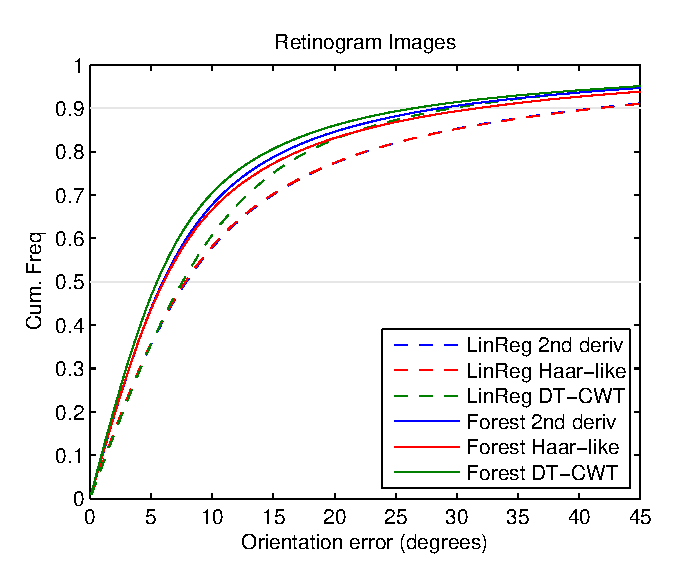
\includegraphics[width=0.48\columnwidth]{\figpath/retina/retinogram_expt} &
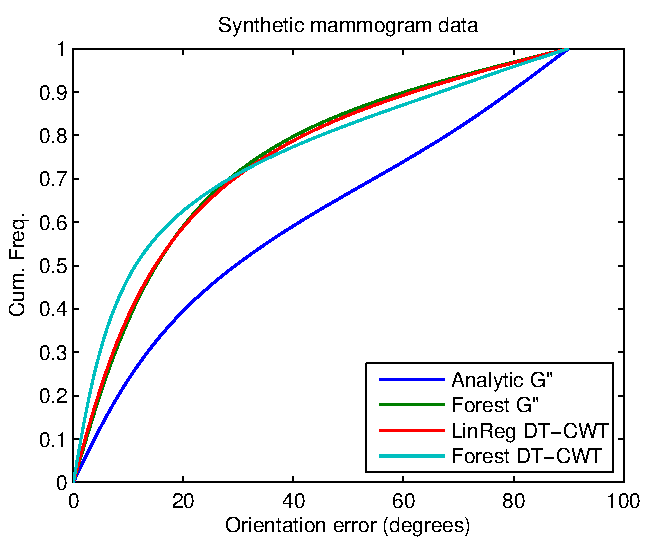
\includegraphics[width=0.48\columnwidth]{\figpath/mammo/mammography_expt} \\
(a) & (b) \\
\end{tabular}
%
\caption{Cumulative frequency of angular error for (a) retinogram images and (b) synthetic mammogram-like images.}
\label{f:cumfreq}
\end{figure}

Comparing performance for the various combinations (\fref{f:cumfreq}a and \tref{t:retinopathy}), we see that in general the analytic methods perform poorly in comparison with the regression approaches, that Random Forests outperform other regression methods and that the \dtcwt~is superior to other feature representations. With the exception of the boosted regressor, the Haar-like approximation exhibited similar performance to the second derivative, suggesting that it may be used effectively in scenarios where efficiency is a concern.

It may be surprising just how poorly the analytic formulations perform in contrast to the regressors. On inspection of the outputs, we see that the monogenic signal (based on first derivatives) does indeed fail at the centre of linear structures. Since, however, many of the vessels in the retinograms are a single pixel in width (such that anywhere on the line is at the centre by definition) the monogenic signal is doomed. The regressors also get some benefit from pooling responses over several pixels.

As noted earlier, when using squared or second derivative responses it is necessary to compute the responses at the two possible solutions to determine which is the correct one. With the Haar-like approximation that combines the response to $\Ixx$ and $\Iyy$, this analytic solution is not available and a regression approach becomes necessary. Also, since the linear regressor minimizes the average error it contains no mechanism for selecting the correct orientation in this way. This is likely to be one reason for its poor performance relative to more sophisticated regressors such as the Random Forest. There is a penalty, however, in efficiency when using complex regressors like the Random Forest.


\subsection{Mammogram-like Images}
\label{s:expts_synth_mammography}
\begin{table}[t]
\centering
\begin{tabular}{l|c c c c}
							& \multicolumn{4}{c}{Feature Type} \\
							& Monogenic		& 2nd deriv.	& Haar				& \dtcwt \\
\hline
\input{mammography_table.txt}
\end{tabular}
%
\caption{Median absolute error (degrees) for combinations of input feature and regressor on 100 synthetic mammogram images.}
\label{t:synth_mammography}
\end{table}

As vessels are often clearly visible in retinograms, we repeated this experiment on a more challenging dataset of synthetic images that realistically approximate the structure of mammographic images. More specifically, we sampled a background by cropping a $512{\times}512$ image region from a real mammogram upon which we superimposed one or more lines of varying orientation, contrast, width and profile (\fref{f:synth_mammography}a). As the lines were synthetic, we had access to both a mask (\fref{f:synth_mammography}b) and ground truth orientation for the superimposed structure.

As in the retinogram experiment, we sampled 200\,000 pixels from such images and computed a feature vector for each with which we trained a regressor. We then applied every trained regressor for every feature type to a fixed set of 100 synthesized images and computed the error at the known foreground pixel positions (\fref{f:synth_mammography}c). As before, Random Forests and the \dtcwt~outperform other methods, though errors were generally higher on account of the more challenging data (\fref{f:cumfreq}b and \tref{t:synth_mammography}). We also note that although the median error for the Random Forest was lower for the \dtcwt~than the second derivatives, the situation was reversed for higher percentiles (\ie~the graphs cross). We care less, however, about differences between errors above a certain threshold (it matters little whether the estimate is out by $60^\circ$ or $70^\circ$ -- they are both terrible estimates) so it may be argued that the Random Forest performs better over the region in which we are interested.

\begin{figure}[t]
\centering
\begin{tabular}{c c c}
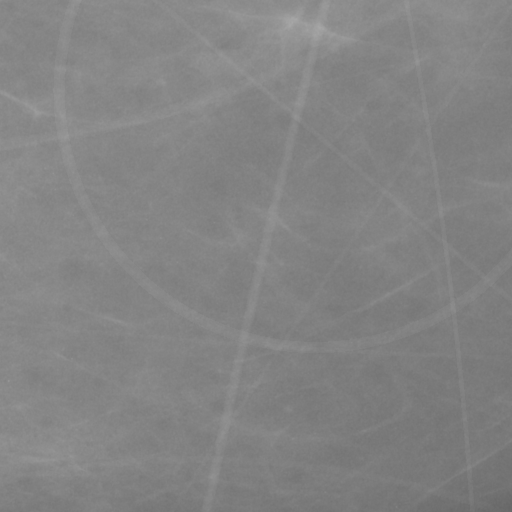
\includegraphics[width=0.3\columnwidth]{\figpath/mammo/synth_lines} &
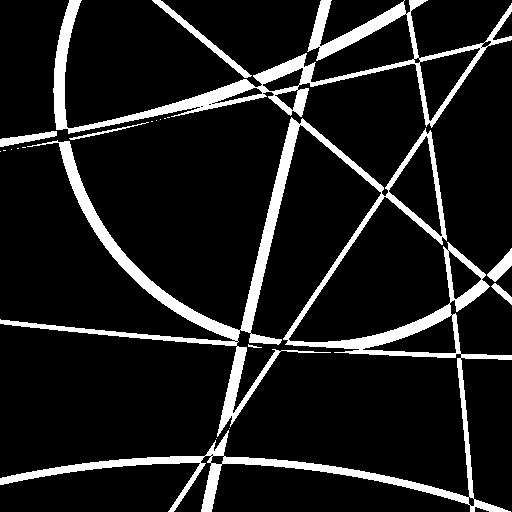
\includegraphics[width=0.3\columnwidth]{\figpath/mammo/synth_mask} &
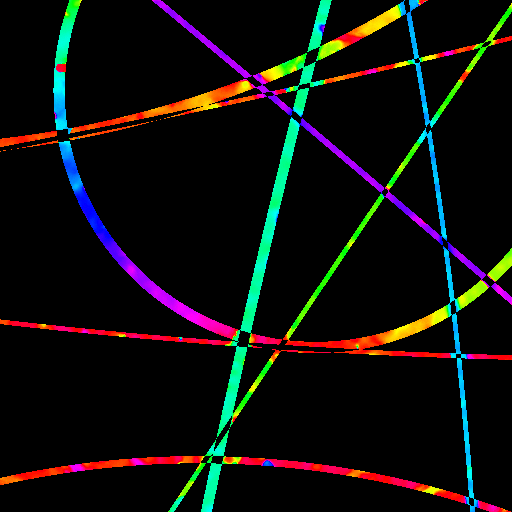
\includegraphics[width=0.3\columnwidth]{\figpath/mammo/synth_result} \\
(a) & (b) & (c)
\end{tabular}
%
\caption{Synthetic mammographic images: %
(a) input image; %
(b) mask indicating pixels belonging to a vessel; %
(c) orientation (indicated by colour) estimated using Random Forest regression over \dtcwt~features. The mask was not used to estimate orientation.%
}
\label{f:synth_mammography}
\end{figure}

\begin{figure}[t]
\centering
\begin{tabular}{c c}
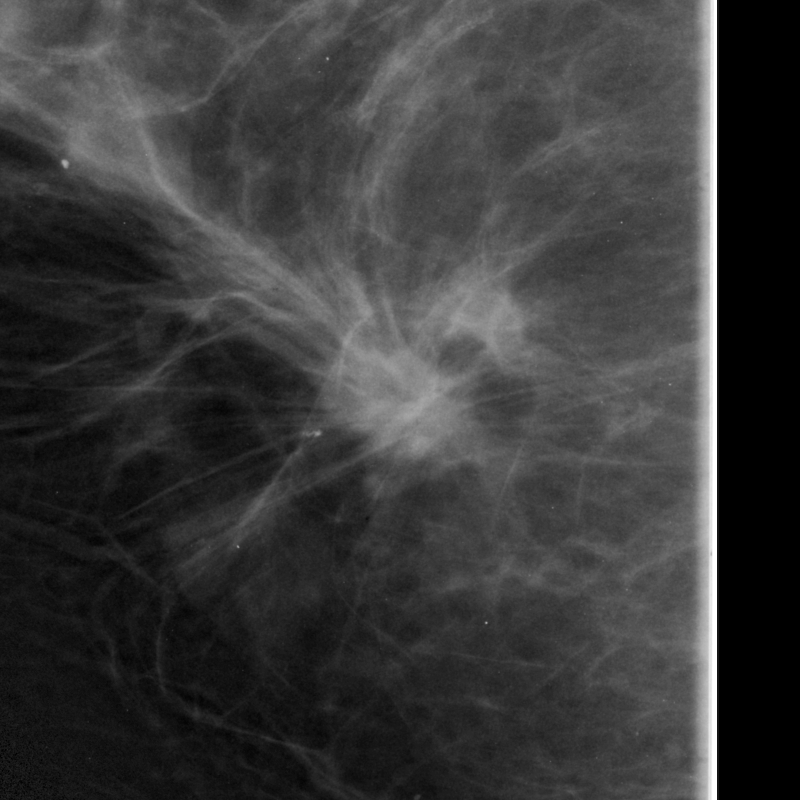
\includegraphics[width=0.3\columnwidth]{\figpath/mammo/024RCC_roi} &
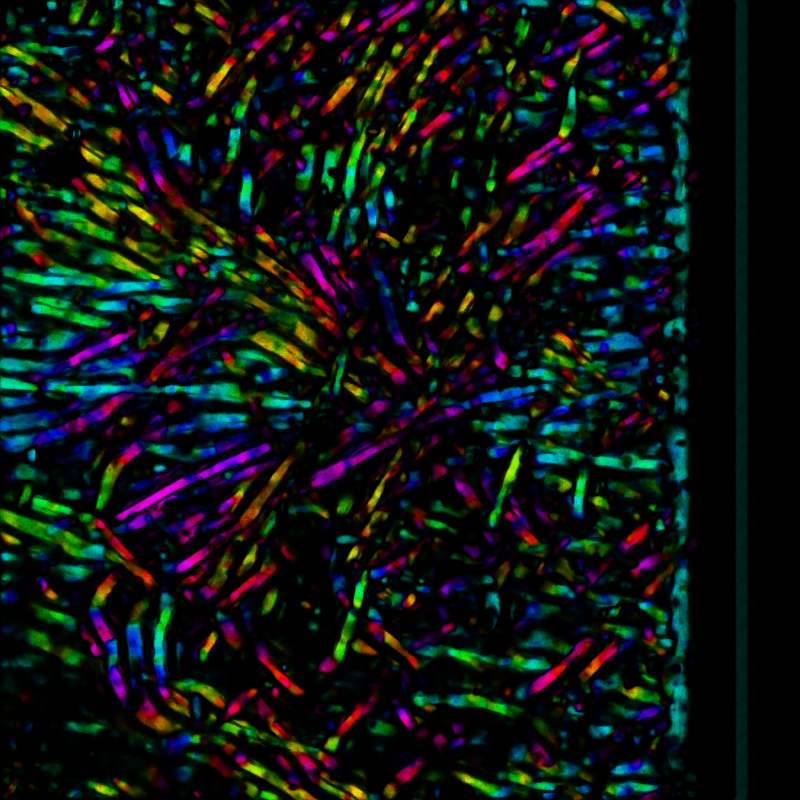
\includegraphics[width=0.3\columnwidth]{\figpath/mammo/024RCC_roi_class_ori_masked} \\
(a) & (b) \\
\end{tabular}
%
\caption{Real mammographic images: %
(a) input image; %
(b) estimated orientation from a Random Forest using \dtcwt~features. Hue indicates the estimated orientation and brightness is determined by the confidence in the estimate (as quantified by the dispersion).}
\label{f:real_mammography}
\end{figure}

% CLAIM: that the separable filters are faster than nonseparable ones (but by how much?)
% CLAIM: that the Haar-like features are faster than separable filtering
In terms of efficiency, we recorded the mean time (using Matlab on a 2.66Ghz, quad-core desktop PC with 3.25Gb RAM) over 20 images for five feature representations: the monogenic signal (2.96\emph{s}); non-separable second derivatives (3.71\emph{s}); separable second derivatives (2.04\emph{s}); their Haar-like approximations (2.35\emph{s}); and the \dtcwt (19.96\emph{s}). Unsurprisingly, under test conditions the separable filters were indeed faster than their non-separable counterparts while the \dtcwt~was an order of magnitude slower than the separable filters. The Haar-like approximations were comparable to but slower than the separable filters, though the separable filters did exploit the built-in (\ie~compiled) convolution functions in Matlab; we expect that an optimized implementation of the Haar-like features would offer similar performance gains as observed in face detection applications~\cite{Viola_Jones_IJCV04}.
%%% This is a pretty weak conclusion to the experiment but the best we can expect at this point. Also, if you need to use a regressor as slow as the RF to get accuracy that is comparable to the analytic second derivatives then the small difference in filtering time becomes irrelevant}

Having trained regressors on synthetic mammogram-like images, we can also apply them to real mammograms. In a region of interest surrounding a spiculated lesion, the linear structures radiating from the central mass are clearly visible when weighted by the confidence in their orientation estimation (\fref{f:real_mammography}).


\subsection{Fingerprint Analysis}
\label{s:expts_fingerprints}
Noting that estimating orientation is of interest to the fingerprint analysis community, we briefly present some results that highlight the difference in performance between using filters based on first and second derivatives, respectively. As discussed earlier, the estimated orientation using gradient based filters~\cite{Bazen_Gerez_TPAMI02,Mei_etal_IVC09} -- the mainstay of fingerprint orientation analysis -- becomes unstable near the centre of a symmetric bar feature (\fref{f:fingerprints}c), whereas a filter based on second derivatives remains stable. There are, however, artefacts around the edges of the ridge features for the second derivative that may suggest a solution based on both types.

\begin{figure}[t]
\centering
\begin{tabular}{c c c}
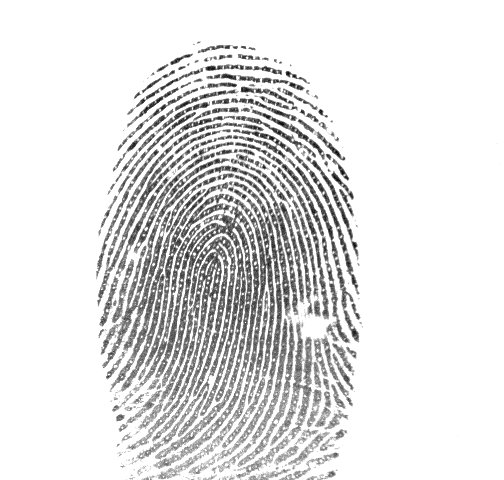
\includegraphics[width=0.3\columnwidth]{\figpath/fingerprint/input} &
%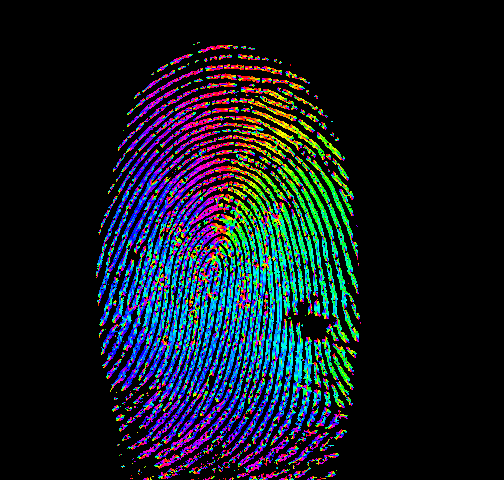
\includegraphics[height=0.15\textheight]{\figpath/fingerprint/ori_1st} &
%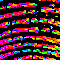
\includegraphics[height=0.15\textheight]{\figpath/fingerprint/ori_1st_zoom} \\
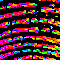
\includegraphics[width=0.3\columnwidth]{\figpath/fingerprint/ori_1st_zoom} &
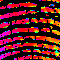
\includegraphics[width=0.3\columnwidth]{\figpath/fingerprint/ori_clover_zoom} \\
(a) & (b) & (c) \\
%&
%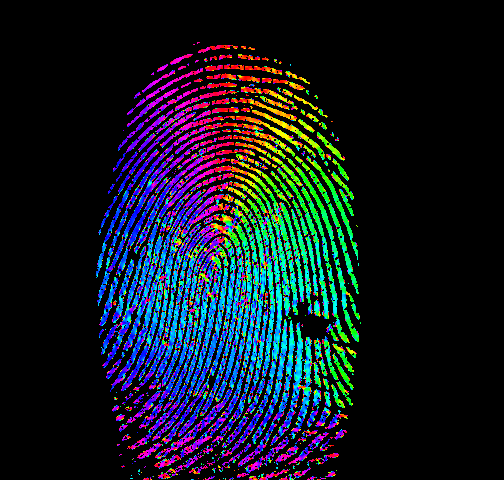
\includegraphics[height=0.15\textheight]{\figpath/fingerprint/ori_clover} &
%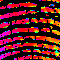
\includegraphics[height=0.15\textheight]{\figpath/fingerprint/ori_clover_zoom} \\
%		& (d) & (e)
\end{tabular}
%
\caption{Fingerprint images: %
(a) input image; %
(b,c) first derivative estimate of orientation with close-up; %
(d-e) second derivative estimate with close-up. Note the high errors at the centre of the ridge for first derivatives and at the edges of the ridge for second derivatives.}
\label{f:fingerprints}
\end{figure}


\section{Discussion}
\label{s:discussion}
\begin{itemize}
\item Combining first and second derivatives: firsts are good at edges, seconds are good at line centres - they complement each other.

\item Discussion about linear regression coefficients: how they take a sinusoidal appearance, how we need to choose between two discrete orientations (which is not possible with a `vanilla' linear regressor)
%
\begin{figure}[t]
	\centering
		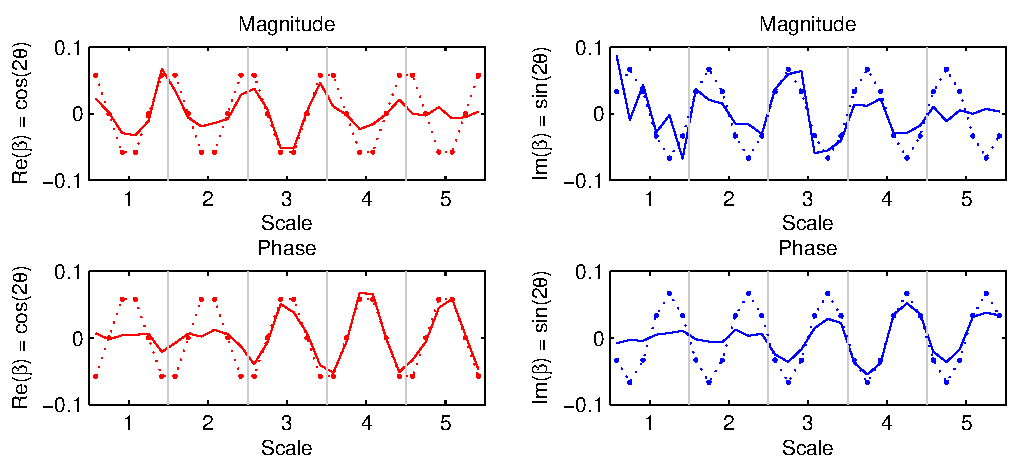
\includegraphics[width=0.9\columnwidth]{\figpath/linreg_coeffs}
	\caption{Linear regression coefficients for (left) $\cos 2\theta$ and (right) $\sin 2\theta$, using (top) response magnitude and (bottom) response phase.}
	\label{f:linreg_coeffs}
\end{figure}

\item Logistic regression can be used to limit the output to -1..+1. Boosted regression implicitly does the same by predicting only what it has seen before. These limits, however, are applied to sinT and cosT independently which means you can still get values outside of the unit circle.

\item Random Forest classifier/regressor has lots of details to get right, not least in making sure that the orientations wrap around correctly. Also differences in how the branches are split etc.

\end{itemize}


\section{Conclusions}
\label{s:conclusions}
From these experiments, we can make several conclusions. First, we see that filters based on first derivatives do indeed perform poorly near the centre of a ridge feature (\fref{f:fingerprints}b); second derivatives are much better, though they result in artefacts at the edges (where we are less concerned). Second, there is potential to approximate the second derivative filter responses with Haar-like features if efficiency is a key concern, though it is less clear how to combine these responses to give a unique solution. Of the filters we tested, we found that the \dtcwt~gave the best results regardless of the regressor used, though was significantly more computationally expensive. Of the regressors we tested, Random Forests performed best and we have provided some insight as to why alternatives (\eg~linear regression) perform less well. We must, however, take care when building regressors for orientation prediction in order to ensure that angles wrap around the circle correctly.


\chapter{Experiments}
We denote the combination of an image representation with a classifier by \emph{representation/classifier} (for example, the \dtcwt{} combined with a Random Forest is denoted by \dtcwt{}/RF).

These learning variants were developed for two reasons: firstly, when analyzing quantitative results for detection performance, they allow us to decouple the effect of random forest learning from the effect due to the type of representation used. 


\section{Datasets}
\subsection{Real Mammograms}
The main purpose of this work was to develop methods for analysing curvilinear structure in mammogram images. To evaluate the algorithms, we took images from a sequential set of 84 abnormal mammograms with biopsy-proven malignancy, drawn from a screening population (Nightingale Breast Centre, South Manchester University Hospitals Trust, UK), and from a set of 89 normal mammograms of the contralateral breasts of the same individuals (where disease was radiologically confirmed to be confined to one breast). All mammograms were digitised to a resolution of $90 \mu\text{m}$ using a Vidar CADPRO scanner. A $4 \by 4$ cm ($512 \by 512$ pixel) patch was then extracted around each abnormality, and a similar patch sampled randomly from each of the normal mammograms (\fref{f:real_examples}). 

For each abnormal patch, an expert radiologist manually annotated some (though not necessarily all) of the spicules associated with the abnormality, giving a total of 555 spicule annotations. Though these expert spicule annotations were not sufficiently accurate to be used directly, we used them as a basis for selecting spicule pixels by initialising a snake~\cite{Kass_etal_IJCV88} with each original annotation, and iterating it to convergence using evidence from the\comment{linear structure probability} image~\cite{Muralidhar_etal_TMI10}. In total, the 555 refined spicule annotations identified 36\,514 spicule pixels. To ensure balanced training sets, we sampled the same number from the normal images.


\subsection{Synthetic Mammogram-like Images}
Given the practical difficulties of obtaining a precise binary labelling of curvilinear structure in mammograms, we generated synthetic images with which to train and evaluate each algorithm\cite{Berks_PhD10}. Specifically, to create each image we again took a $4 \by 4$ cm ($512 \by 512$ pixel) region from a real mammogram with 256 grey levels, and processed it\comment{be more specific} to remove linear structures, leaving only the coarse background texture with local image noise across all frequencies. We then superimposed several linear structures with randomly chosen parameters (orientation, width, peak intensity, \comment{curvature,?} profile shape, etc) onto the background. The result was an image whose statistics were close to a real mammogram but with known line parameters (\fref{f:synthetic_responses}).

In this manner, we generated 10\,460 training images and 4\,903 test image patches from 72 (30) normal mammograms. The line parameters were drawn from probability distributions that were chosen to mimic what is found in real mammograms:

\begin{itemize}
\item orientations were drawn from a uniform distribution over the range [0, $\pi$] radians.
\item widths were drawn from a uniform distribution over [4, 16] pixels.
\item peak intensity [1,255] grey-levels (relative to images scaled 0 - 255) from an exponential distribution with half-width 4 grey-levels; 
\item profile shape $S$ determined by the equation $S = s + (1-s) \sin(x)$ for offsets $x \in (0,\pi)$, where the 'squareness' parameter $s$\comment{could be confused with scales defined elsewhere} determines how close the shape is to a pure half-cycle $\sin$ or a rectangle and is drawn uniformly from [0,1]. 
\end{itemize}

The literature suggests (and this is borne out by our experience) that the best performance is obtained by training with a balanced dataset - in this case with the same number of foreground (curvilinear structure) and background examples. Having created these images, therefore, we sampled feature vectors at pixels on the centrelines of the superimposed linear structure, and an equal number of `background' pixels to serve as positive and negative training sets, respectively.\comment{for detection, of course} 

When testing an algorithm on an unseen image, we compute the output for every pixel in the image.

To construct the orientation regression random forests, we sample points randomly from line pixels in the synthetic images (the orientation of a background pixel is undefined).

During training, backgrounds were randomly sampled from the 10460 training patches and a single line was added to the centre of the patch. These images were produced 'on-the-fly' during each tree-building step of random forest construction and no permanent set was maintained. (We simply generated images until we had the desired 200k points, then built the tree; we did this for 200 trees.)

For testing, 100 backgrounds were randomly selected from the test patches. To each, multiple lines were added sequentially, with the number and position of lines varying randomly.

Note that all synthetic lines used were straight lines. We conducted experiments explicitly using curved structures, however as there was no performance difference between training on curved or straight lines when detecting curved lines, it was decided that including curves was unnecessary.

All forests were constructed with 200 trees and following published guidelines~\cite{Breiman_ML01}. However, rather than using a single set of training data from which samples were drawn with replacement (\ie bootstrapping), we used our method for randomly generating unique synthetic lines images to construct a new training sample at each tree-building step. For detection, each sample comprised 100k curvilinear structure pixels and 100k background pixels, while for orientation regression we used 200k pixels all belonging to curvilinear structure. 


\subsection{Retinal Images}
The publicly available DRIVE dataset~\cite{Staal_etal_TMI04} contains 40 full colour retinogram images (\fref{f:retinography}a) of $565 \by 584$ pixels, each with a hand-labelled mask that indicates vessel pixels (\fref{f:retinography}b), and split into training (images 21-40) and test (images 01-20) sets. The masks provided ground truth for the presence of a line in the image, and by skeletonizing the mask we approximated ground truth orientation, $\theta_{gt}$, for every labelled pixel.\comment{It is questionable how well this constitutes ground truth}

For training, we transformed all images to monochrome via a weighted sum of the three RGB channels (though using only the green channel is also popular). We then selected 200\,000 vessel pixels randomly over the training set and computed filter responses for every selected pixel.

\begin{figure}[t]
\centering
\begin{tabular}{c c c}
\includegraphics[width=0.3\columnwidth]{\figpath/retina/02_test} &
\includegraphics[width=0.3\columnwidth]{\figpath/retina/02_manual1} &
\includegraphics[width=0.3\columnwidth]{\figpath/retina/002_orientation_masked} \\
%\includegraphics[height=0.15\textheight]{\figpath/retina/002_abs_error} \\
(a) & (b) & (c) \\
\end{tabular}
%
\caption{Estimating orientation in retinography: %
(a) input image; %
(b) ground truth mask indicating pixels belonging to a vessel; %
(c) orientation (indicated by colour) estimated using linear regression over \dtcwt{} features. The mask was not used to estimate orientation. %
%(c) magnitude of error (note the regions of high error at points of bifurcation.)
}
\label{f:retinography}
\end{figure}


\subsection{Fingerprint Images}
\comment{Where did this data come from?}
Noting that estimating orientation is of interest to the fingerprint analysis community, we briefly present some results that highlight the difference in performance between using filters based on first and second derivatives, respectively. As discussed earlier, the estimated orientation using gradient based filters~\cite{Bazen_Gerez_TPAMI02,Mei_etal_IVC09} -- the mainstay of fingerprint orientation analysis -- becomes unstable near the centre of a symmetric bar feature (\fref{f:fingerprints}c), whereas a filter based on second derivatives remains stable. There are, however, artefacts around the edges of the ridge features for the second derivative that may suggest a solution based on both types.

\begin{figure}[t]
\centering
\begin{tabular}{c c c}
\includegraphics[width=0.3\columnwidth]{\figpath/fingerprint/input} &
%\includegraphics[height=0.15\textheight]{\figpath/fingerprint/ori_1st} &
%\includegraphics[height=0.15\textheight]{\figpath/fingerprint/ori_1st_zoom} \\
\includegraphics[width=0.3\columnwidth]{\figpath/fingerprint/ori_1st_zoom} &
\includegraphics[width=0.3\columnwidth]{\figpath/fingerprint/ori_clover_zoom} \\
(a) & (b) & (c) \\
%&
%\includegraphics[height=0.15\textheight]{\figpath/fingerprint/ori_clover} &
%\includegraphics[height=0.15\textheight]{\figpath/fingerprint/ori_clover_zoom} \\
%		& (d) & (e)
\end{tabular}
%
\caption{Fingerprint images: %
(a) input image; %
(b,c) first derivative estimate of orientation with close-up; %
(d-e) second derivative estimate with close-up. Note the high errors at the centre of the ridge for first derivatives and at the edges of the ridge for second derivatives.}
\label{f:fingerprints}
\end{figure}


\subsection{Nailfold Capillaroscopy Images}



\section{Detecting Linear Structures}
In our first set of experiments, we investigate the ability of each image representation and classification method to detect the presence of a line (\ie~a bar) in the image. For this task, we used a binary label (present \vs not present) as the target we aimed to predict.

Having trained a classifier using the synthetic data, we can classify feature vectors extracted about every pixel in a synthetic or real mammogram image to obtain a line probability image (using the probabilistic labelling scheme as opposed to a hard binary classification).

Monogenic, Linop and Gaussian are representative of the current state of the art in line detection, and all permit an analytic approach to line detection.

Secondly, unlike their original variants, Monogenic/RF, Linop/RF and Gaussian/RF can be used in the spicule classification experiment.

By forming such a feature vector at each pixel in a training set of ground-truth labelled images, we can obtain a large set of data which can be used to train a random forest classifier to differentiate between linear structures and background. In constructing the best detector, this discriminative approach takes account of the characteristics of the background pixels as well as the curvilinear structure pixels.

Details on the composition of feature vectors for each representation type are given below. Note for all methods, the number of scales used $s$ and the neighbourhood size $w$ were empirically tested to select the best combination for each method. In each case, we tried $s$ = 3, 4, 5, 6 and $w$ = 1, 3. For reasons of space, results are shown only for the best combination in each method.

\begin{itemize}
\item	DT-CWT/RF: images were decomposed using the DT-CWT to $s$ scales. Neighbourhoods of interpolated phase and magnitude coefficients were extracted in each of the 6 oriented subbands producing a feature vector of $12 w^2 s$ elements.
\item	Monogenic/RF: the monogenic signal was extracted across $s$ scales, with the initial wavelength set at $\lambda$ = 4 pixels. Neighbourhoods of phase, amplitude and orientation values were computed giving a total feature size of $3 w^2 s$. 
\item	Linop/RF: 8 oriented line filters were computed at each scale. Collecting neighbourhoods of the oriented filter responses produced $8 w^2 s$ elements in each feature vectors.
\item	Gaussian/RF: for the Gaussian 2nd derivative method, the three directional derivatives were applied to an image at each scale. The standard deviation of the smallest kernel was 1 pixel, subsequent kernels increased by a factor of 2 at each scale. As with Monogenic/RF this resulted in feature vectors with $3 w^2 s$ elements.
\end{itemize}

For testing, feature vectors for each representation were extracted at all pixels in the 100 synthetic test images. The classification and regression forests were then used to compute a line detection score (the proportion of votes for the curvilinear structure class) . Example results of line detection are shown in~\ref{f:synthetic_responses}.


\begin{figure}
\centering
\begin{tabular}{c c c c}
\includegraphics[width=\qtrcol]{\figpath/ipmi/line512_003} &
\includegraphics[width=\qtrcol]{\figpath/ipmi/line512_003_lines} &
\includegraphics[width=\qtrcol]{\figpath/ipmi/line512_003_gaussian} &
\includegraphics[width=\qtrcol]{\figpath/ipmi/line512_003_monogenic} \\
(a) & (b) & (c) & (d) \\
\includegraphics[width=\qtrcol]{\figpath/ipmi/line512_003_rf_191905} &
\includegraphics[width=\qtrcol]{\figpath/ipmi/line512_003_rf_191961} &
\includegraphics[width=\qtrcol]{\figpath/ipmi/line512_003_rf_233141} &
\includegraphics[width=\qtrcol]{\figpath/ipmi/line512_003_rf_191960} \\
(e) & (f) & (g) & (h)
\end{tabular}
%
\caption{Synthetic test image and corresponding filter responses: (a) original image; (b) Linop; (c) Gaussian; (d) Monogenic; (e) DT-CWT/RF; (f) Linop/RF; (g) Gaussian/RF; (h) Monogenic/RF.}
\label{f:synthetic_responses}
\end{figure}


\begin{figure}
\centering
\begin{tabular}{c c c c}
\includegraphics[width=\qtrcol]{\figpath/ipmi/mass028} &
\includegraphics[width=\qtrcol]{\figpath/ipmi/mass028_linop} &
\includegraphics[width=\qtrcol]{\figpath/ipmi/mass028_gaussian} &
\includegraphics[width=\qtrcol]{\figpath/ipmi/mass028_monogenic} \\
(a) & (b) & (c) & (d) \\
\includegraphics[width=\qtrcol]{\figpath/ipmi/mass028_dt} &
\includegraphics[width=\qtrcol]{\figpath/ipmi/mass028_rf_linop_w1l5} &
\includegraphics[width=\qtrcol]{\figpath/ipmi/mass028_rf_gaussian} &
\includegraphics[width=\qtrcol]{\figpath/ipmi/mass028_rf_monogenic_w3l4} \\
(e) & (f) & (g) & (h)
\end{tabular}
%
\caption{Mammogram region containing malignant spiculated mass and corresponding filter responses: (a) original image; (b) Linop; (c) Gaussian; (d) Monogenic; (e) \dtcwt{}/RF; (f) Linop/RF; (g) Gaussian/RF; (h) Monogenic/RF.}
\label{f:real_responses}
\end{figure}


\begin{figure}
\centering
\begin{tabular}{c c c}
\includegraphics[width=0.33\columnwidth]{\figpath/ipmi/line_detection_roc} &
\includegraphics[width=0.33\columnwidth]{\figpath/ipmi/rf_spic_1_6}
\end{tabular}
%
\caption{Receiver operating characteristic (ROC) curves for different curvilinear structure detection methods; centre: Cumulative distribution functions (CDF) of errors in orientation estimation for the different methods; right: ROC curves for spicule classification.}
\label{f:detection_roc}
\end{figure}

ROC curves for the seven methods tested are shown in~\ref{f:} 2, using the known ground-truth for the test images to define pixels on the centrelines of curvilinear structures as foreground, and pixels lying outside the structures as background. Areas under the ROC curves and detection sensitivities at a fixed specificity of 90\% are shown in~\ref{t:}. 

These results show that the four learning methods perform significantly better than the three prescriptive methods (with the exception of orientation computation in Monogenic/RF). \dtcwt{}/RF is significantly the strongest performing for both line detection and orientation estimation, followed by Linop/RF then Gaussian/RF.

As expected, because Linop, of the three prescriptive methods, discards the highest proportion of filter responses, Linop/RF gains the most from training. This highlights the ability of the random forests to extract useful information from a rich local description of image content, and while we do not have a prescriptive variant to compare it to, we believe this shows the importance of training in maximizing the benefit of using the \dtcwt{}. We also note that the added information that can be gained from the \dtcwt representation results from an increase in the richness of the local description of texture and is not due to increasing the support of the descriptor. Indeed, as described above we tested all representations over an equivalent range of filter scales so that the same image support was available to each method.

Assessing the detection results visually, it would appear that the outputs of the learning based methods (and particularly \dtcwt{}/RF, Linop/RF and Gaussian/RF) are similar to the output of synthetic data while capturing the key curvilinear structures in the real regions. This would suggest our model for producing synthetic lines generates good data from which to train random forests for real images. Of course validating this hypothesis is important and we are currently working on a quantitative evaluation of the methods in real data when used, for example, as part of a larger lesion detection scheme.


\section{Classifying Linear Structures}
Classification is of interest when it is important to distinguish between subtly different structures which may be present within the same image - for example, rivers and roads

When classifying between different types of linear structure, our hypothesis is that the cross-sectional intensity profiles of different structures vary in systematic ways~\cite{Zwiggelaar_etal_TMI04} that can be used to discriminate between classes.

, and that profile shape is effectively captured by the \dtcwt{} coefficients - particularly in the phase components. 

We concentrated on the task of distinguishing between spicules (an indicator of malignancy) and other curvilinear structures.  To create a balanced training set we sampled feature vectors from the same number of pixels in a set of normal mammogram patches, such that the distribution of curvilinear structure probabilities was the same as for the spicule training set. Using this balanced training set, we built a random forest classifier to perform spicule/non-spicule classification.

The literature on classifying curvilinear structures in mammograms is much more limited. We are aware of the work of Zwiggelaar et al~\cite{Zwiggelaar_etal_TMI04}, which demonstrated the feasibility of distinguishing between different types of structure using cross-sectional profiles obtained from manually annotated curvilinear structures, but did not obtain very satisfactory results when the method was fully automated.  We recently reported preliminary classification (but not detection) results using our current approach~\cite{Chen_etal_IWDM10}.


The four learning-based methods were also applied to the problem of spicule/non-spicule classification. Feature vectors were formed as above, and random forest classifiers were trained using balanced spicule/non-spicule training data.

To make effective use of the available data, we used a 10-fold cross-validation design. The set of normal and abnormal regions were divided into 10 groups so that the total number of normal and spicule pixels in each group were as close as possible to a 10th of the total and no two views from the same case were included in different groups. The samples in each group were then classified using a random forest trained on the samples from the remaining 9 groups. The classification results from each group were pooled to generate an unbiased class probability for each sampled pixel. These probabilities were used to compute an ROC curve for each training regime, and the area under the curve (Az) was computed and used as a measure of classification performance. The ROC curves and Az values for the three methods are shown in \ref{f:} 2 and \ref{t:} 2. These results demonstrate a clear advantage for \dtcwt{}/RF. As might be expected, because the Linop and Gaussian representations do not really capture profile shape, they perform significantly worse that the two representations that include phase.

In addition to computing a class vote for spicule membership at only those pixels in the selected training sets, the forests we have constructed can be used to compute results for whole region in each cross-fold group. Typical qualitative \dtcwt{}/RF results for a normal and abnormal region are shown in \ref{f:} 4. In the left column, the original regions are shown. The spiculations of the mass are clear and well defined, particularly to the south-east of the central mass. In the normal region, there are a set of structures that intersect in an approximate radial pattern that may trigger a feature detector erroneously. In the right column, the predicted spicule class membership is shown as hue varying from cyan (normal) to pink (spicule), modulated by the output of the \dtcwt{}/RF detection method. Note how the linear structures in the region of the mass are deemed highly likely to be spicules, while those in the normal region are not. This shows excellent promise as a means of providing a relevance measure to methods for abnormality detection.

\begin{figure}
\centering
\begin{tabular}{c c c}
\includegraphics[width=0.33\columnwidth]{\figpath/ipmi/orientation_estimation_cdf} &
\end{tabular}
\end{figure}

\begin{table}
\caption{Results for spicule classification. For every algorithm, we show the area under the ROC curve ($A_z$)}
\label{t:spicule_classification}
%
\begin{tabular}{l c}
Algorithm
		& ROC $A_z$ \\
\hline
\dtcwt{}/RF ($w$ = 1, $s$ = 6, all orientations)
		& 0.761$\pm$0.0034 \\
Monogenic/RF ($w$ = 1, $s$ = 5, 8 orientations)
		& 0.748$\pm$0.0035 \\
Gaussian/RF ($w$ = 1, $s$ = 5, $\sigma_{min}$ = 1)
		& 0.718$\pm$0.0037 \\
Linop/RF ($w$ = 1, $s$ = 5, $\lambda$ = 4)
		& 0.716$\pm$0.0037 \\
\end{tabular}
\end{table}

\begin{figure}
\centering
\begin{tabular}{c c}
\includegraphics[width=\qtrcol]{\figpath/ipmi/mass046} &
\includegraphics[width=\qtrcol]{\figpath/ipmi/norm068} \\
(a) & (b) \\
\includegraphics[width=\qtrcol]{\figpath/ipmi/spic_prob_mass046_a} &
\includegraphics[width=\qtrcol]{\figpath/ipmi/spic_prob_norm068_a} \\
(c) & (d)
\end{tabular}
%
\caption{Regions depicting (a) malignant and (b) normal tissue. The corresponding spicule classification results are depicted in (c,d) using hue to indicate abnormality -- ranging from cyan (normal) to pink (spicule) -- and intensity to indicate the line detection output from the \dtcwt{} method.}
\label{f:spicule_classification}
\end{figure}


\section{Estimating Orientation}
In addition to detecting curvilinear structure in mammograms, for many subsequent analysis tasks (\eg~detecting abnormal patterns of structure indicative of disease) it is equally important that we can make accurate estimates of orientation. As with detection, rather than doing this prescriptively, we pose the problem as a regression task in which we learn how patterns of \dtcwt{} coefficients correspond to structures at varying orientations. Feature vectors of \dtcwt{} coefficients are formed as in section 2.1, with the difference that the image ground truth specifies the orientation of a pixel as opposed to its class membership. A random forest regressor can then be trained to predict the orientation of any pixel given its \dtcwt{} representation.

Curvilinear structures are important in many applications of computer vision, including aerial image analysis (roads, rivers, railways), fingerprint analysis (ridges) and medical image analysis (blood vessels, ducts). As a result, there is an extensive literature on detecting such structure~\cite{Papari_Petkov_IVC11}. The literature on estimating the local orientation of curvilinear structure is more limited though the problem is equally important, for example as a basis for non-maximal suppression (centre-line detection) and for characterising properties such as tortuosity (\eg~of blood vessels).

In mammography, malignant lesions often exhibit linear structures (known as spicules) that form a radial pattern around the central mass. Detecting linear structures and determining their orientation~\cite{Zwiggelaar_etal_MIA99,Zwiggelaar_etal_TMI04} can therefore indicate points where they converge and thus whether a mass or architectural distortion is present~\cite{Karssemeijer_teBrake_TMI96,Rangayyan_Ayres_MBEC06}. In other medical applications such as retinography (\fref{f:retinography}), the rate of change of orientation (\ie~tortuosity) of blood vessels can serve as a diagnostic indicator of vascular disease~\cite{Hart_etal_IJMI99}; though studies have shown that vessels can be detected and segmented~\cite{Staal_etal_TMI04,Ricci_Perfetti_TMI07,Dabbah_etal_MICCAI10}, few have addressed the problem of measuring their orientation and quantifying tortuosity.

Similarly, automatic fingerprint analysis typically begins by computing the orientation at each pixel via gradient-based filtering, often followed by some smoothing over a local patch~\cite{Bazen_Gerez_TPAMI02,Mei_etal_IVC09}. This orientation field is often parameterized -- via `phase portraits'~\cite{Li_etal_PR06} or polynomial approximation~\cite{Gu_etal_PR04}, for example -- to capture and interpret the underlying properties of the fingerprint such as its `singular points' where the orientation is no longer defined (\eg~at a delta or the centre of a whorl). Though smoothing orientation estimates at a local patch have been the subject of several investigations~\cite{Kass_Witkin_CVGIP87,Rao_Jain_TPAMI92,Perona_TIP98}, we deal only with the initial step of estimating orientation at every pixel.

In this paper we revisit the problem of orientation estimation, reviewing the basic theory, extending the state-of-the-art, and providing the results of extensive evaluation using both real and realistic synthetic images. The first step in estimating orientation usually involves applying a set of linear filters to the image, generally at multiple scales and orientations. As we will show later, the choice of filter-bank has a significant influence on both computational efficiency, and estimation accuracy. Our contribution is to explore the similarities and differences between different approaches, and provide empirical evidence of which work best in practice.

Given a set of filter-bank outputs, the second step in estimating orientation is to combine them in some way. There are two basic approaches: to find the scale at which the total magnitude of response is greatest, and combine the different filter responses at that scale analytically~\cite{Karssemeijer_teBrake_TMI96,Mei_etal_IVC09}; or to use a regression learning approach to combine the filter responses across all scales and orientations~\cite{Berks_etal_IPMI11}. Our contribution is to explore the technical details of orientation regression and provide a comprehensive evaluation of different combinations of filter-bank and analytic/regression methods. Overall we show that an approach based on combining dual-tree complex wavelet filtering with random forest regression achieves significantly better results than any of the other state-of-the-art approaches tested.

During testing, we applied each regressor in turn to estimate the orientation, $\theta_{est}$, at every pixel for every test image and computed the orientation error with respect to ground truth,
%
\begin{equation}
	\theta_{err} = \frac{\angle(2\theta_{est}-2\theta_{gt})}{2}
\end{equation}

\noindent only at labelled vessel pixels in the test image mask (\fref{f:retinography}c).\comment{A reviewer will probably complain that this is cheating and that we should have used a classifier}

These results show that the four learning methods perform significantly better than the three prescriptive methods (with the exception of orientation computation in Monogenic/RF). \dtcwt{}/RF is significantly the strongest performing for both line detection and orientation estimation, followed by Linop/RF then Gaussian/RF.

===

In our first set of experiments, we present a quantitative evaluation of the three regressors on real retinography images and mammogram-like data for which we have ground truth. We also present qualitative results on some real mammography images and fingerprint images for which ground truth was not available.


\subsection{Real Retinographic Images}
\label{s:expts_retinography}

\begin{table}[b]
\centering
\begin{tabular}{l|c c c c}
							& \multicolumn{4}{c}{Feature Type} \\
							& Monogenic		& 2nd deriv.	& Haar				& \dtcwt{} \\
\hline
\input{retinogram_table.txt}
\end{tabular}
%
\caption{Median absolute error (degrees) for combinations of input feature and regressor on the DRIVE database of retinal images (images 01-20).}
\label{t:retinopathy}
\end{table}

\begin{figure}
\centering
\begin{tabular}{c c}
\includegraphics[width=0.48\columnwidth]{\figpath/retina/retinogram_expt} &
\includegraphics[width=0.48\columnwidth]{\figpath/mammo/mammography_expt} \\
(a) & (b) \\
\end{tabular}
%
\caption{Cumulative frequency of angular error for (a) retinogram images and (b) synthetic mammogram-like images.}
\label{f:cumfreq}
\end{figure}

Comparing performance for the various combinations (\fref{f:cumfreq}a and \tref{t:retinopathy}), we see that in general the analytic methods perform poorly in comparison with the regression approaches, that Random Forests outperform other regression methods and that the \dtcwt{} is superior to other feature representations. With the exception of the boosted regressor, the Haar-like approximation exhibited similar performance to the second derivative, suggesting that it may be used effectively in scenarios where efficiency is a concern.

It may be surprising just how poorly the analytic formulations perform in contrast to the regressors. On inspection of the outputs, we see that the monogenic signal (based on first derivatives) does indeed fail at the centre of linear structures. Since, however, many of the vessels in the retinograms are a single pixel in width (such that anywhere on the line is at the centre by definition) the monogenic signal is doomed. The regressors also get some benefit from pooling responses over several pixels.

As noted earlier, when using squared or second derivative responses it is necessary to compute the responses at the two possible solutions to determine which is the correct one. With the Haar-like approximation that combines the response to $\Ixx$ and $\Iyy$, this analytic solution is not available and a regression approach becomes necessary. Also, since the linear regressor minimizes the average error it contains no mechanism for selecting the correct orientation in this way. This is likely to be one reason for its poor performance relative to more sophisticated regressors such as the Random Forest. There is a penalty, however, in efficiency when using complex regressors like the Random Forest.


\subsection{Mammogram-like Images}
\label{s:expts_synth_mammography}
\begin{table}[t]
\centering
\begin{tabular}{l|c c c c}
							& \multicolumn{4}{c}{Feature Type} \\
							& Monogenic		& 2nd deriv.	& Haar				& \dtcwt{} \\
\hline
\input{mammography_table.txt}
\end{tabular}
%
\caption{Median absolute error (degrees) for combinations of input feature and regressor on 100 synthetic mammogram images.}
\label{t:synth_mammography}
\end{table}

As vessels are often clearly visible in retinograms, we repeated this experiment on a more challenging dataset of synthetic images that realistically approximate the structure of mammographic images. More specifically, we sampled a background by cropping a $512{\times}512$ image region from a real mammogram upon which we superimposed one or more lines of varying orientation, contrast, width and profile (\fref{f:synth_mammography}a). As the lines were synthetic, we had access to both a mask (\fref{f:synth_mammography}b) and ground truth orientation for the superimposed structure.

As in the retinogram experiment, we sampled 200\,000 pixels from such images and computed a feature vector for each with which we trained a regressor. We then applied every trained regressor for every feature type to a fixed set of 100 synthesized images and computed the error at the known foreground pixel positions (\fref{f:synth_mammography}c). As before, Random Forests and the \dtcwt{} outperform other methods, though errors were generally higher on account of the more challenging data (\fref{f:cumfreq}b and \tref{t:synth_mammography}). We also note that although the median error for the Random Forest was lower for the \dtcwt{} than the second derivatives, the situation was reversed for higher percentiles (\ie~the graphs cross). We care less, however, about differences between errors above a certain threshold (it matters little whether the estimate is out by $60^\circ$ or $70^\circ$ -- they are both terrible estimates) so it may be argued that the Random Forest performs better over the region in which we are interested.

\begin{figure}[t]
\centering
\begin{tabular}{c c c}
\includegraphics[width=0.3\columnwidth]{\figpath/mammo/synth_lines} &
\includegraphics[width=0.3\columnwidth]{\figpath/mammo/synth_mask} &
\includegraphics[width=0.3\columnwidth]{\figpath/mammo/synth_result} \\
(a) & (b) & (c)
\end{tabular}
%
\caption{Synthetic mammographic images: %
(a) input image; %
(b) mask indicating pixels belonging to a vessel; %
(c) orientation (indicated by colour) estimated using Random Forest regression over \dtcwt{} features. The mask was not used to estimate orientation.%
}
\label{f:synth_mammography}
\end{figure}

\begin{figure}[t]
\centering
\begin{tabular}{c c}
\includegraphics[width=0.3\columnwidth]{\figpath/mammo/024RCC_roi} &
\includegraphics[width=0.3\columnwidth]{\figpath/mammo/024RCC_roi_class_ori_masked} \\
(a) & (b) \\
\end{tabular}
%
\caption{Real mammographic images: %
(a) input image; %
(b) estimated orientation from a Random Forest using \dtcwt{} features. Hue indicates the estimated orientation and brightness is determined by the confidence in the estimate (as quantified by the dispersion).}
\label{f:real_mammography}
\end{figure}

% CLAIM: that the separable filters are faster than nonseparable ones (but by how much?)
% CLAIM: that the Haar-like features are faster than separable filtering
In terms of efficiency, we recorded the mean time (using Matlab on a 2.66Ghz, quad-core desktop PC with 3.25Gb RAM) over 20 images for five feature representations: the monogenic signal (2.96\emph{s}); non-separable second derivatives (3.71\emph{s}); separable second derivatives (2.04\emph{s}); their Haar-like approximations (2.35\emph{s}); and the \dtcwt{} (19.96\emph{s}). Unsurprisingly, under test conditions the separable filters were indeed faster than their non-separable counterparts while the \dtcwt{} was an order of magnitude slower than the separable filters. The Haar-like approximations were comparable to but slower than the separable filters, though the separable filters did exploit the built-in (\ie~compiled) convolution functions in Matlab; we expect that an optimized implementation of the Haar-like features would offer similar performance gains as observed in face detection applications~\cite{Viola_Jones_IJCV04}.
%%% This is a pretty weak conclusion to the experiment but the best we can expect at this point. Also, if you need to use a regressor as slow as the RF to get accuracy that is comparable to the analytic second derivatives then the small difference in filtering time becomes irrelevant}

Having trained regressors on synthetic mammogram-like images, we can also apply them to real mammograms. In a region of interest surrounding a spiculated lesion, the linear structures radiating from the central mass are clearly visible when weighted by the confidence in their orientation estimation (\fref{f:real_mammography}).


\subsection{Fingerprint Analysis}
\label{s:expts_fingerprints}


\section{Discussion}
\label{s:discussion}
\begin{itemize}
\item Combining first and second derivatives: firsts are good at edges, seconds are good at line centres - they complement each other.

\item Discussion about linear regression coefficients: how they take a sinusoidal appearance, how we need to choose between two discrete orientations (which is not possible with a `vanilla' linear regressor)
%
\begin{figure}[t]
	\centering
		\includegraphics[width=0.9\columnwidth]{\figpath/linreg_coeffs}
	\caption{Linear regression coefficients for (left) $\cos 2\theta$ and (right) $\sin 2\theta$, using (top) response magnitude and (bottom) response phase.}
	\label{f:linreg_coeffs}
\end{figure}

\item Logistic regression can be used to limit the output to -1..+1. Boosted regression implicitly does the same by predicting only what it has seen before. These limits, however, are applied to sinT and cosT independently which means you can still get values outside of the unit circle.

\item Random Forest classifier/regressor has lots of details to get right, not least in making sure that the orientations wrap around correctly. Also differences in how the branches are split etc.

\end{itemize}

and orientation (the mean output of each regression tree, with appropriate angular wrapping at 0\deg and 180\deg) at each pixel

For orientation, only pixels belonging to curvilinear structures (although not necessarily at the centerline) were included in the results. The absolute differences between the predicted and known orientations (with appropriate angle wrapping) were taken, and used to generate cumulative distribution functions of orientation errors for each method, as shown in~\ref{f:}. The mean absolute errors of the estimated orientations are also included in~\ref{t:}.

The orientation results for both Monogenic and Monogenic/RF were surprisingly poor. Counter-intuitively, visual analysis of the test outputs showed that the Monogenic methods performed particularly badly at the exact centerline of curvilinear structures, where an essentially random orientation appeared to be returned. This is in contrast to the other tested methods that, as expected, performed strongest along the centerlines of structures. Computing estimation errors at pixels belonging to structures but not lying on the centerline produces a small improvement in the results (mean absolute errors of 32.55\deg and 29.39\deg for the RF and prescriptive variant respectively), though even then performance lags behind the other tested methods and of course in a real image we do not know the precise location of structure centerlines. Determining why orientations are estimated so poorly by the monogenic signal at the centre of structures, where in theory the signal is strongest, may warrant further investigation.




In terms of applying the learning methods to real images, it is worth noting how the methods scale with increasing image size - particularly above the point at which the set of feature vectors for all image pixels can be stored in working memory. For the \dtcwt{}, provided the initial decomposition can be stored in memory (which due to its low-redundant decimating construction is possible even for full size mammograms of the order 3000x2400 pixels) then interpolated coefficients can be efficiently sampled to generate feature vectors for block-wise regions of the image. Each block of feature vectors can be classified by the forest and cleared from working from memory storing only the output of the forest. In this way only a small overhead is introduced for block-wise classifying the image. However, for the other methods it becomes necessary to interleave the decomposition of the image with the sampling of feature vectors. For example, it may be necessary to apply the filters at a single scale, extract features for that scale for a particular block of the image, filter at the next scale and extract those features, and so on. Of course, when the complete feature vectors for a single block have been classified, the process repeats. Thus a large image may in fact end up by decomposed many times over introducing a large computational overhead for block-wise processing. The point at which this cost occurs will depend on the size of the image and the type of representation used. Obviously the cost is worst for Linop which requires storing 8 (\ie the number orientations) full copies of the image at each scale, compared to just 3 for the Gaussian and Monogenic methods.



\begin{table}
\centering
\caption{Line detection and orientation computation results. For every algorithm, we present the area under the ROC curve ($A_z$), the sensitivity at 90\% specificity, and the mean absolute error of the orientation estimate.}
\label{t:line_detection}
%
\begin{tabular}{l c c c}
Algorithm	
		& $A_z$							& Sens. \@ 90\% spec. & MAE \\
\hline
\dtcwt{}/RF ($w$ = 1, $s$ = 5)												
		& 0.923$\pm$0.00036	& 0.792 							& 15.88 \\
Linop/RF ($w$ = 1, $s$ = 5, 8 orientations)				
		& 0.911$\pm$0.00048	& 0.757								& 19.35 \\
Gaussian/RF ($w$ = 1, $s$ = 4, $\sigma_{min}$ = 1)
		& 0.901$\pm$0.00048	& 0.731								& 21.37 \\
Monogenic/RF ($w$ = 1, $s$ = 4, $\lambda$ = 4)
		& 0.868$\pm$0.00045	& 0.643								& 33.73 \\
Monogenic ($s$ = 3, $\lambda$ = 4)									
		& 0.818$\pm$0.00055	& 0.547								& 30.86 \\
Gaussian ($s$ = 4, $\sigma_{min}$ = 1)							
		& 0.813$\pm$0.00053	& 0.533								& 24.27 \\
Linop ($s$ = 5, 8 orientations)										
		& 0.737$\pm$0.00060	& 0.413								& 29.32 \\
\end{tabular}
\end{table}



\section{Discussion}
The results of our experimental evaluation are extremely encouraging, and represent a significant improvement over the current state of the art. 

Although learning accounts for a significant part of this improvement, the choice of representation is also important and will have a different effect on performance depending on the task in hand. For example, constructing a representation based on the raw responses to Linop filters produces features that are excellent for estimating structure orientation but provide less information for determining structure shape and thus type. 

Conversely, features formed from the monogenic signal are good at determining structure type - most likely because of the inclusion of the phase measure - while they perform relatively poorly at detection and orientation estimation. 

For these reasons, it seems fair to conclude that the \dtcwt{} provides the best all round representation. It produced the strongest performance for all three tasks (curvilinear structure detection, orientation estimation and spicule classification). Moreover, the \dtcwt{} incurs the least overhead when working with full-size real images that require block-wise classification/regression. For example, initial tests show that the structure detection and orientation regression can be performed on a full-size (~3000 x 2400 pixels) mammogram in ~1hr 30mins.

We show that, overall, our approach is significantly better than the current state-of-the-art, and that we can distinguish effectively between curvilinear structures associated with malignancy (spicules) and those associated with normal structure (vessels, ducts etc).
\chapter{Detecting Spiculated Masses}

\section{Related Work}
Kupinski and Giger~\cite{Kupinski_Giger_TMI98} present a method for computing the boundary of the lesion, given that you know its centre in advance. It's basically a thresholding algorithm with some constraints to make the boundary smoother (I guess you'd get something similar by applying a snake~\cite{Kass_etal_IJCV88}.

Interestingly, Hand \etal~\cite{Hand_etal_CBR79} look for both circumscribed and spiculated masses also using the idea that gradients are oriented in different directions for the two types. Not bad for 1979, given that they digitized the films using a video camera and framegrabber.


\subsection{Spiculated Masses}
Ball and Bruce~\cite{Ball_Bruce_EMBC07} use level sets to segment the spiculated mass from the background. They start with an initialization from a previous work~\cite{Ball_PhD07} which is in turn based on Reyer's paper~\cite{Zwiggelaar_etal_TMI04} and Linop~\cite{Dixon_Taylor_IPC79}. Wait a minute. They're lying. They don't use level sets at all -- just a horribly complex sequence of image processing steps.


\subsection{Mass Classification}
Baeg and Kehtarnavaz~\cite{Baeg_Kehtarnavaz_ELCVIA02} present a method that that classifies masses into \emph{benign} or \emph{malignant}, depending on their image properties. They compute two features: denseness and (confusingly) `architectural distortion', and feed these into a neural network. It looks like their classifier boils down to `malignant masses are brighter and less round than benign ones'.


\section{Detecting Curvilinear Structure}
When looking for a spiculated mass, it is not unusual to look for its characteristic pattern of spicules radiating from a central mass. Since the central mass is not always present (in which case the abnormality presents itself as an \emph{architectural distortion}), we can instead look for the radial pattern of the spicules alone. The usual approach is to apply a classifier of some description that looks for curvilinear structure and look for a focal point all lines in a region of interest.

Karssemeijer's method is a prime example~\cite{Karssemeijer_teBrake_TMI96}. There are, however, a number of points to be made about this:

\begin{itemize}
\item This requires a line strength threshold above which pixels are classified as `line'; it is not clear what this threshold should be. 

\item I'm not entirely convinced that taking the maximum over all scales is a good thing. In fact, the whole point of using RFs with \dtcwt{} coefficients is to avoid doing this.

\item Line strength is not necessarily a good indicator of line presence. For example, a perfectly circular disc will give a strong response yet its orientation is not well defined. We could consider points where there is a big difference between maximum and minimum responses -- this is probably a stronger indication of a linear structure with well-defined orientation.

\item Black-on-white lines are discarded, even though they have the correct orientation and may be valid estimates of oriented texture (even though they are not spicules). 

\item Another criteria for elimination is that a gradient operator gives a strong response \emph{and} the orientation estimate from 1st derivatives and 2nd derivatives agree (indicating an edge); since we know that 2nd derivatives are rubbish at edges, however, the pixels closest to the edge usually are not discarded (though other points close to the edge are).

\item The 1st derivative gradient operator is applied at a single large scale (much larger than the 2nd derivative operators). I find this a little weird and may give funny results for edge detection.

\item The second derivative filters do not have the same power and therefore are not scale invariant. They should be adapted to avoid bias between levels.

\item True lines are characterized by a strong negative response at the line centre, with a fairly strong positive response at a known distance along the normal on both sides. 
\end{itemize}


\section{Karssemeijer's Method}
\subsection{Region Of Interest}
Outer radius, inner radius and size of `bullseye': I think the inner radius should be big enough to mask out the mass, and the outer radius about twice the size. The bullseye is around half the inner radius in my experiments. Karssemeijer uses different parameters.

There is also the open question of whether the measure should be scale invariant (it isn't). There are arguments both ways here.

\subsection{Pixel Weights}
The weights of individual pixels can be defined in different ways, each with a sensible argument. The one Karssemeijer uses has a bullseye and points are counted as `positive' if their line passes through the bullseye; this puts high weight on points far from the centre (since it is more unusual for one far away to be correctly aligned). Another defines a fixed angular error such that points are weighted equally. A third could be to put more weight on points that are close to the centre (since those points should be directed to the centre whereas we expect points far from the mass to be more randomly oriented).

\subsection{Sensitivity to Line Maps}
The selected points appear to have a larger effect on g2d estimated orientations than those from the Random Forest. We're not sure why.

\subsection{Assumed Background Distribution}
It should be possible to model the background distribution as a spatially varying quantity, given normal images with which to train. This would be instead of the assumed uniform distribution over orientation which is not true for regions close to the skin.

\chapter{Asymmetry Detection}

\section{Related Work}
Ferrari \etal~\cite{Ferrari_etal_TMI01} use Gabor filters to estimate the orientation of texture in the image, computing responses at a number of scales, applying PCA somewhere (they don't say why this is sensible), some thresholding (not sure why exactly). They compute a rose diagram (an orientation histogram) ``that represents the difference between the rose diagrams
computed for the left and right mammograms'' and compute three features: entropy (I think they have high/low entropy confused), mean orientation and variance (or dispersion, in which I don't think they account for wraparound). They then classify these 3-vectors using linear discriminant analysis (or ``the Bayesian linear classifier'' as they call it). They reckon that using the mean orientation alone over the whole breast is enough to discriminate between symmetric and asymmetric cases. This is based on a sample of 40 image pairs (20 normal, 20 abnormal). Interestingly, they get sensitivity and specificity values like 77.3\% and 71.4\% and 23.8\% -- with only 40 image pairs, shouldn't these numbers all be to the nearest 2.5\%? It's also difficult to accept that a single architectural distortion in one breast is sufficient to generate a significant difference in global statistics over the whole breast -- on a local level, however, I can believe it.


\subsection{Registration}
In order to compute breast asymmetry, it is sensible to first align the two images:

\begin{itemize}
\item \textbf{Between-side:} This is the easiest case and there must be several examples.
\item \textbf{Between-view:} This is a more interesting but much more difficult scenario where we associate every point in the CC view with a line in the MLO view (or vice versa)~\cite{Kita_etal_CVPR98,vanEngeland_Karssemeijer_IWDM06}
\item \textbf{Between-patient:} For the same view, I suspect this falls in between the previous two scenarios in terms of difficulty. It is, however, difficult to see why you would want to do this.
\end{itemize}

van Engeland and Karssmeijer~\cite{vanEngeland_etal_TMI03} present a comparison of four registration tehcniques: nipple alignment; centre of mass alignment; mutual information-based alignment; and nonrigid image warping (via a thin plate spline). They conclude that nonrigid warping is rubbish, nipple alignment isn't great and the other two are about the same. Correctly segmenting the pectoral muscle and background was found to have a significant effect in several cases.

Kita \etal~\cite{Kita_etal_CVPR98} attempt the difficult between-view case by building a 3D model of the breast from the two projected outlines and applying a model of how the breast might deform under compression. van Engeland and Karssemeijer~\cite{vanEngeland_Karssemeijer_IWDM06} do something similar though I'd need to check details.

Lau and Bischof~\cite{Lau_Bischof_CBR91} is an old paper that aligns the breast via an affine transform computed from three control points estimated from the boundary. They then compute a brightness measure and a roughness measure at each pixel. Combining these (along with their ratio) and a measure of directionality to suppress responses near highly oriented structures (\eg~vessels) they estimate an map of asymmetry between the two breasts.

Wirth \etal~\cite{Wirth_etal_IPA99} use Radial Basis Function as a nonlinear interpolant to achieve nonrigid warping of one breast onto another.

Tahmoush and Samet~\cite{Tahmoush_Samet_SPIE06} locate suspicious points via an interest point detector. What they do then is anyone's guess -- something about a `separator' (classifier?) that uses the difference in distribution of suspicious points between the contralateral breasts to diagnose cancer. I kind of understand what they mean but they are far too vague on details. They proceed to publish an almost identical study (and I mean ``identical'' in the word-for-word sense) in IWDM~\cite{Tahmoush_etal_IWDM06}.

Yin \etal~\cite{Yin_etal_JDI94} use a registration technique described elsewhere before computing something akin to the difference image. They then process this image to look for localized masses.

Miller and Astley~\cite{Miller_Astley_BMVC93} suggest ignoring registration for global asymmetry detection and instead focussing on segmentation such that measures are computed only for regions of the same type of breast tissue. This seems a very sensible approach for global measures at least.


\subsection{Histograms}
Rangayyan \etal~\cite{Rangayyan_etal_JEI07} is probably the closest we'll get to something beyond the usual register-subtract approach. They compute line orientations using Gabor filters and compare, in addition to Hu moments, the statistics of histograms over line orientations between left and right breasts. They use a linear or quadratic classifier to discriminate between healthy and abnormal cases based on subsets of these features, achieving best accuracy with a quadratic classifier and four features (none of which are the Hu moments).

A key question that often arises is that of which histogram distance measure is best. The Earth Mover's Distance (EMD), derived from the \emph{transportation problem}, is often used as one of the better ones for reasons described in Rubner \etal~\cite{Rubner_etal_IJCV00} (which also contains descriptions of some other measures). One problem with the EMD is that it requires iterative optimization to compute which makes it considerably slower than most other metrics. A fast approximation was proposed by Indyk and Thaper~\cite{Indyk_Thaper_SCTV03} and subsequently used for matching contours~\cite{Grauman_Darrell_CVPR04}. A comprehensive list of many distance measures (many of which can be shown to be equivalent) is given by Cha~\cite{Cha_IJMMMAS07}.

Many papers try to model the distribution of a histogram in a Euclidean space, often with a Gaussian distribution (\eg~\cite{Broadhurst_etal_DSSCV05}). This is wrong (and~\cite{Broadhurst_etal_DSSCV05} admit so) whereas other papers look at the problem from a statistical point of view to model the likelihood properly~\cite{Vermeesch_JGR05}. Modelling the distribution of a set of histograms is apparently discussed by Weltje~\cite{Weltje_ESR02} but it's long and I haven't read it yet.

Two more papers may be worth considering. Kadir and Brady~\cite{Kadir_Brady_TR05} present a method for estimating histograms that is less sensitive to quantizing effects; it works by interpolating the sampled signal and computing the histogram of the resulting continuous function. This is more stable than simply histogramming the sampled points, though I suspect it is less accurate in certain circumstances (\ie~a bias-variance tradeoff). Finally, Aherne \etal discuss the merits of the Bhattacharyya distance as the optimal histogram measure~\cite{Aherne_etal_Kybernetika97} (this paper was pointed out to me by Neil Thacker).


\section{Vector Quantization}
One method for determining the similarity of left and right breasts reduces each image to a feature vector with an associated distance measure. In this experiment, we select random patches from normal mammograms, and compute a spatially varying histogram over orientation for each point.

\begin{figure}[t]
	\centering
		\def\figpath{\figroot/asymmetry}
		\includegraphics[height=0.3\textheight]{\figpath/roi_full}
		\includegraphics[height=0.3\textheight]{\figpath/roi_zoom}
%
	\caption{Region of Interest overlaid on full image and a close-up.}
	\label{f:logpolar_roi}
\end{figure}

More specifically, we define a log-polar region of interest (\ie~divided linearly by angle and logarithmically by radius) that divides the region into a number of cells (\fref{f:logpolar_roi}). We compute the histogram over orientation for all pixels contained in each cell and concatenate into a single feature vector that captures not only the distribution of orienation within the region of interest but also how it varies spatially (similar to the \emph{f2} feature in Karssemeijer's method~\cite{Karssemeijer_teBrake_TMI96}).

\begin{figure}[t]
	\centering
		\def\figpath{\figroot/asymmetry/centre_001}
		\includegraphics[width=0.15\columnwidth]{\figpath/sample_001}
		\includegraphics[width=0.15\columnwidth]{\figpath/sample_002}
		\includegraphics[width=0.15\columnwidth]{\figpath/sample_003}
		\includegraphics[width=0.15\columnwidth]{\figpath/sample_004}
		\includegraphics[width=0.15\columnwidth]{\figpath/sample_005}
		\includegraphics[width=0.15\columnwidth]{\figpath/sample_006}%
		\vspace{2pt}%
		\def\figpath{\figroot/asymmetry/centre_031}
		\includegraphics[width=0.15\columnwidth]{\figpath/sample_001}
		\includegraphics[width=0.15\columnwidth]{\figpath/sample_002}
		\includegraphics[width=0.15\columnwidth]{\figpath/sample_003}
		\includegraphics[width=0.15\columnwidth]{\figpath/sample_004}
		\includegraphics[width=0.15\columnwidth]{\figpath/sample_005}
		\includegraphics[width=0.15\columnwidth]{\figpath/sample_006}%
		\vspace{2pt}%
		\def\figpath{\figroot/asymmetry/centre_047}
		\includegraphics[width=0.15\columnwidth]{\figpath/sample_001}
		\includegraphics[width=0.15\columnwidth]{\figpath/sample_002}
		\includegraphics[width=0.15\columnwidth]{\figpath/sample_003}
		\includegraphics[width=0.15\columnwidth]{\figpath/sample_004}
		\includegraphics[width=0.15\columnwidth]{\figpath/sample_005}
		\includegraphics[width=0.15\columnwidth]{\figpath/sample_009}%
		\vspace{2pt}
		\def\figpath{\figroot/asymmetry/centre_046}
		\includegraphics[width=0.15\columnwidth]{\figpath/sample_001}
		\includegraphics[width=0.15\columnwidth]{\figpath/sample_002}
		\includegraphics[width=0.15\columnwidth]{\figpath/sample_003}
		\includegraphics[width=0.15\columnwidth]{\figpath/sample_004}
		\includegraphics[width=0.15\columnwidth]{\figpath/sample_005}
		\includegraphics[width=0.15\columnwidth]{\figpath/sample_006}
%
	\caption{Image patches corresponding to four different histogram vector quantization codebook entries.}
	\label{f:codebook_patches}
\end{figure}

Given a set of sampled histograms from normal mammograms, we then cluster the histograms (via K-means) to generate a `codebook' of orientation patterns. Each codebook vector should represent a local orientation pattern in the image (\fref{f:codebook_patches}).

A new image can then be reduced to a feature vector by selecting points at random, computing their orientation histograms, assigning each to a cluster centre, and computing the histogram over cluster assignments. The intuition is that symmetric breasts will exhibit a similar distribution over orientation patterns, such that the distances between the left and right histograms will be, on average, lower in normal (\ie~symmetric) cases than in abnormal (asymmetric) ones.

\begin{figure}[t]
	\centering
		\def\figpath{\figroot/asymmetry}
		\includegraphics[width = 0.9\columnwidth]{\figpath/graphs}
%
	\caption{Distributions of left-right distance measure for normal and abnormal pairs, viewed as individual samples, a histogram, and a cumulative histogram.}
	\label{f:vq_distances}
\end{figure}

To test the intuition, we computed the left-right distance for all normal pairs (neither of which was used to generate the codebook) and all abnormal pairs. We see a small difference in distribution between normal and abnormal groups, but not enough to build a classifier on (\fref{f:vq_distances}).


\section{Direct Matching}
In another experiment, we looked at matching individual regions of the two images based on a histogram distance between reference and target points. I didn't figure out where to take it from there -- maybe a total distance between left and right, possibly with a Markov Random Field prior to encourage comparison between points that are qualitatively in the same place (\fref{f:hist_matches}).

\begin{figure}[t]
	\centering
	\def\figpath{\figroot/asymmetry}
	\begin{tabular}{c c}
	\begin{minipage}[c]{0.5\columnwidth} 
		\includegraphics[width=\columnwidth]{\figpath/044LCC_match_matches} 
	\end{minipage}
	\begin{minipage}[c]{0.5\columnwidth}
		\includegraphics[width=\columnwidth]{\figpath/044LCC_match_hist3d}
	\end{minipage}
	\end{tabular} 
%
	\caption{(left) Matched points on left and right breast images for 044CC; (right) visualization of histograms as points in a plane with matched histograms linked by a line.}
	\label{f:hist_matches}
\end{figure}


\section*{Acknowledgements}
We thank Nick Kingsbury for the DT-CWT Matlab toolbox. Mammograms were provided by the Nightingale Breast Centre, South Manchester University Hospitals Trust, UK and were annotated by Dr Caroline Boggis and Dr Rumana Rahim. This work was funded by EPSRC grant EP/E031307/1.

\bibliographystyle{plain}
\bibliography{%
./bib/_aliases,%
./bib/mobio,%
./bib/mammography,%
./bib/ml,%
./bib/local}

\end{document}